\documentclass[12pt]{article}

\usepackage{sbc-template}
\usepackage{graphicx,url}
\usepackage[utf8]{inputenc}
\usepackage[T1]{fontenc}
\usepackage[brazil]{babel}
\usepackage{amsmath,amssymb}
\usepackage{float}
\usepackage{multirow}
% sem hyperref: com ele, o sbc-template.sty redefine \@ e quebra o babel nas versões recentes do LaTeX

% pseudocódigos (o ambiente "algorithm" não está disponível nesta instalação)
\floatstyle{ruled}
\newfloat{algoritmo}{tbp}{loa}
\floatname{algoritmo}{Algoritmo}
\newcommand{\linha}[1]{\par\noindent\hangindent=4em\hangafter=1\makebox[1.4em][r]{\scriptsize #1}\hspace{0.6em}}

% gerado por relatorio/gerar_figuras.py -- não editar
\newcommand{\nInst}{27}
\newcommand{\nInviaveis}{1}
\newcommand{\nTotal}{28}
\newcommand{\gapIni}{12,29}
\newcommand{\gapFin}{2,12}
\newcommand{\gapFinMax}{17,13}
\newcommand{\gapLb}{2,56}
\newcommand{\melhoria}{8,75}
\newcommand{\tempoMedio}{3,18}
\newcommand{\otimos}{1}
\newcommand{\refOtima}{7}
\newcommand{\abaixoUm}{21}
\newcommand{\melhorQueMip}{8}
\newcommand{\semMip}{0}
\newcommand{\nComparaModelo}{24}
\newcommand{\reducaoModelo}{29,5}
\newcommand{\reducaoModeloMin}{-1,6}
\newcommand{\reducaoModeloMax}{62,2}
\newcommand{\tempoMax}{40,74}
\newcommand{\tempoMaxId}{I25}
\newcommand{\tConstrMax}{0,036}
\newcommand{\cvIni}{0,082}
\newcommand{\cvIniMax}{0,476}
\newcommand{\cvFinMax}{0,000}
\newcommand{\nExec}{270}
\newcommand{\piorId}{I02}
\newcommand{\piorGap}{17,13}
\newcommand{\folgaMin}{2,1}
\newcommand{\folgaMax}{23,4}
\newcommand{\Mmin}{100}
\newcommand{\Mmax}{6798}
\newcommand{\Nmin}{5}
\newcommand{\Nmax}{20}
\newcommand{\fracSobreMin}{39}
\newcommand{\fracSobreMax}{100}
\newcommand{\sobrecargaMax}{12,1}
\newcommand{\nInviavelEscola}{3}
\newcommand{\inviaveisEscola}{I01, I11, I21}
\newcommand{\reducaoModeloMinId}{I05}
\newcommand{\idExemplo}{I02}
\newcommand{\idInstUm}{I04}
\newcommand{\idInstDois}{I07}
\newcommand{\idDoisUmUm}{I05}
\newcommand{\idGrupo}{I26}
\newcommand{\idInviavel}{I28}
\newcommand{\idLenta}{I25}
\newcommand{\idFechou}{I19}
\newcommand{\gapExemplo}{17,1}
\newcommand{\refExemplo}{839,98}
\newcommand{\finalExemplo}{983,84}
\newcommand{\reducaoExemplo}{17,0}
\newcommand{\gapInstUm}{11,0}
\newcommand{\refInstUm}{884,54}
\newcommand{\finalInstUm}{981,94}
\newcommand{\reducaoInstUm}{25,1}
\newcommand{\gapInstDois}{9,5}
\newcommand{\refInstDois}{922,89}
\newcommand{\finalInstDois}{1010,19}
\newcommand{\reducaoInstDois}{18,1}
\newcommand{\gapDoisUmUm}{7,2}
\newcommand{\refDoisUmUm}{1850,33}
\newcommand{\finalDoisUmUm}{1984,45}
\newcommand{\reducaoDoisUmUm}{-1,6}
\newcommand{\gapGrupo}{0,1}
\newcommand{\refGrupo}{959,73}
\newcommand{\finalGrupo}{960,53}
\newcommand{\reducaoGrupo}{6,0}
\newcommand{\gapLenta}{0,0}
\newcommand{\refLenta}{7426,28}
\newcommand{\finalLenta}{7426,28}
\newcommand{\reducaoLenta}{54,7}
\newcommand{\gapFechou}{0,0}
\newcommand{\refFechou}{101847,79}
\newcommand{\finalFechou}{101847,79}
\newcommand{\reducaoFechou}{0,9}
\newcommand{\coberturaInst}{10}
\newcommand{\coberturaMax}{5}
\newcommand{\corrTempoTipos}{0,96}
\newcommand{\corrTempoM}{0,31}
\newcommand{\movsTiposLenta}{134}
\newcommand{\movsNQuatroLenta}{24}
\newcommand{\movsNCincoLenta}{110}
\newcommand{\folgaFechou}{23,4}
\newcommand{\escolasFechadas}{2}
\newcommand{\nInstDois}{28}
\newcommand{\nExecDois}{280}
\newcommand{\reducaoDois}{3,48}
\newcommand{\reducaoDoisMin}{0,02}
\newcommand{\reducaoDoisMinId}{I13}
\newcommand{\reducaoDoisMax}{29,8}
\newcommand{\reducaoDoisMaxId}{I02}
\newcommand{\nPioraDois}{0}
\newcommand{\nReducaoUm}{15}
\newcommand{\maioresReducoesDois}{I02, I04, I07, I01, I06}
\newcommand{\maioresReducoesMmax}{382}
\newcommand{\nGrandes}{20}
\newcommand{\nGrandesAbaixoUm}{11}
\newcommand{\reducaoRuimMin}{2,9}
\newcommand{\reducaoRuimMax}{29,8}
\newcommand{\gapLbUm}{5,95}
\newcommand{\gapLbDois}{1,52}
\newcommand{\fechadoDois}{73,8}
\newcommand{\melhoriaDois}{7,64}
\newcommand{\tempoMedioDois}{2,52}
\newcommand{\tempoMaxDois}{21,95}
\newcommand{\tempoMaxDoisId}{I25}
\newcommand{\cvFinDoisMax}{0,000}
\newcommand{\divididasDois}{43,5}
\newcommand{\partNSeis}{3,0}
\newcommand{\finalInviavelDois}{841,58}
\newcommand{\gapLbInviavelDois}{0,4}
\newcommand{\divididasInviavelDois}{14}
\newcommand{\finalExemploDois}{690,75}
\newcommand{\reducaoExemploDois}{29,8}
\newcommand{\divididasExemploDois}{23}
\newcommand{\gapLbExemplo}{63,5}
\newcommand{\gapLbExemploDois}{14,8}


\sloppy

\title{Heurística construtiva e busca em vizinhança variável\\
  para a localização de locais de prova}

% TODO: nomes e e-mails dos integrantes do grupo
\author{Integrante 1\inst{1}, Integrante 2\inst{1}, Integrante 3\inst{1}}

\address{Departamento de Ciência da Computação -- Universidade Federal de Juiz de Fora (UFJF)\\
  Juiz de Fora -- MG -- Brasil
  \email{\{integrante1,integrante2,integrante3\}@estudante.ufjf.br}
}

\begin{document}

\maketitle

\begin{abstract}
  This report addresses the exam location problem of a university admission exam, a variant of the
  single source capacitated facility location problem in which every candidate must be assigned to a
  school offering his or her exam type. Each classroom applies a single exam type and each school
  offers at most $K$ types, with $K \in \{1, 2\}$ given as a parameter ($K = 1$ is the original
  problem). We propose a two-phase constructive heuristic (school and room typing followed by a
  static-regret allocation with a restricted candidate list) and a variable neighborhood descent with
  seven neighborhoods. With one type per school, on the \nInstUm{} feasible instances of the class,
  the method ends, on average, \gapFinUm\% above the best known value (\gapLbUm\% above a lower
  bound), improving the initial solution by \melhoriaUm\% in \tempoMedioUm{} seconds per run on
  average. Allowing two types per school makes \nInstDois{} instances feasible and reduces the total
  distance by \reducao\% on average.
\end{abstract}

\begin{resumo}
  Este relatório trata do problema de localização de locais de prova de um processo seletivo, uma
  variante do problema de localização de facilidades capacitadas com fonte única em que cada
  candidato deve ser alocado a uma escola que ofereça o seu tipo de prova. Cada sala aplica um único
  tipo de prova e cada escola oferece no máximo $K$ tipos, com $K \in \{1, 2\}$ passado como
  parâmetro ($K = 1$ é o problema original). Propomos uma heurística construtiva em duas fases
  (escolha dos tipos das escolas e das salas, seguida de alocação por arrependimento estático com
  lista restrita de candidatos) e uma descida em vizinhança variável com sete vizinhanças. Com um
  tipo por escola, nas \nInstUm{} instâncias viáveis da turma, o método termina, em média,
  \gapFinUm\% acima do melhor valor conhecido (\gapLbUm\% acima de um limite inferior), melhora a
  solução inicial em \melhoriaUm\% e leva \tempoMedioUm{} segundos por execução, em média. Permitir
  dois tipos por escola torna \nInstDois{} instâncias viáveis e reduz a distância total em
  \reducao\%, em média.
\end{resumo}

% =====================================================================================
\section{Introdução}

Todo ano, processos seletivos como o Programa de Ingresso Seletivo Misto (PISM) da UFJF precisam
decidir em quais escolas aplicar as provas e para qual escola enviar cada candidato. Os candidatos
fazem provas de tipos diferentes (módulos e áreas), uma sala não pode aplicar dois tipos de prova ao
mesmo tempo e cada escola tem um número limitado de lugares. Uma alocação ruim obriga milhares de
candidatos a atravessar a cidade, enquanto uma boa alocação reduz deslocamentos, atrasos e custos
de transporte.

O problema foi estudado por \cite{oliveira2021}, que o modelam como uma variante do
\emph{Single Source Capacitated Facility Location Problem} (SSCFLP): cada candidato é atendido por
um único local, os locais têm capacidade e só podem oferecer um tipo de prova. Este trabalho propõe
uma abordagem heurística para o problema, composta por:
\begin{itemize}
  \item uma heurística construtiva em duas fases que sempre gera uma solução viável quando a
    instância tem solução (Seção~\ref{sec:construtivo});
  \item sete estruturas de vizinhança, combinadas numa descida em vizinhança variável (VND)
    \cite{mladenovic1997} (Seção~\ref{sec:busca});
  \item um estudo experimental comparando os resultados com um modelo de programação inteira e com
    um limite inferior (Seções~\ref{sec:experimentos} e~\ref{sec:resultados}), com o número máximo
    de tipos de prova por escola (1 ou 2) como parâmetro do programa.
\end{itemize}

O relatório prioriza a justificativa das decisões tomadas. A Seção~\ref{sec:problema} define o
problema e a interpretação adotada; a Seção~\ref{sec:instancias} caracteriza as instâncias, cujas
propriedades motivam as decisões seguintes; a Seção~\ref{sec:exemplo} mostra um exemplo passo a
passo; a Seção~\ref{sec:ruim} discute os casos em que a abordagem não vai bem; e a
Seção~\ref{sec:conclusao} conclui.

% =====================================================================================
\section{Descrição do problema}\label{sec:problema}

\subsection{Elementos}

Considere um conjunto de candidatos $C$ ($|C| = M$), um conjunto de escolas $L$ ($|L| = N$), cada
escola $j$ com um conjunto de salas $R_j$, sendo $q_r$ a capacidade da sala $r$, e o conjunto de
tipos de prova $T = \{\mathrm{M1}, \mathrm{M2}, \mathrm{M3e}, \mathrm{M3s}, \mathrm{M3h},
\mathrm{M3d}\}$. Cada candidato $i$ tem um tipo de prova $\tau(i) \in T$ e $d_{ij}$ é a distância
do candidato $i$ à escola $j$. A capacidade da escola é $Q_j = \sum_{r \in R_j} q_r$. Nenhuma
escola vem com tipo definido: o tipo é decisão do modelo.

\subsection{Interpretação adotada: salas com um tipo, escolas com até $K$ tipos}\label{sec:interpretacao}

O enunciado estabelece que cada local de prova oferece apenas um tipo de exame. Adotamos como
\textbf{local de prova a escola} e acrescentamos duas regras:
\begin{enumerate}
  \item \textbf{Cada sala aplica um único tipo de prova.} É a restrição física do processo real:
    todos os candidatos de uma sala fazem a mesma prova, com o mesmo tempo e o mesmo fiscal. Por
    isso nenhuma sala é dividida entre tipos.
  \item \textbf{Cada escola oferece no máximo $K$ tipos de prova}, com $K \in \{1, 2\}$ escolhido
    por parâmetro do programa (\texttt{-{}-tipos-por-escola}). Os tipos da escola são os tipos das
    suas salas. Com $K = 1$ (o padrão) todas as salas da escola aplicam a mesma prova, que é
    exatamente o problema do enunciado. Com $K = 2$ a escola pode receber dois tipos, em salas
    diferentes; isso modela uma organização em que cada escola tem uma ou duas coordenações de prova,
    e mede quanto a restrição de um tipo por escola custa em distância.
\end{enumerate}
Os resultados principais usam $K = 1$; a Seção~\ref{sec:tipos-por-escola} compara com $K = 2$.

\subsection{Formulação}

Com as variáveis $x_{ij} = 1$ se o candidato $i$ é alocado à escola $j$, $y_{jt} = 1$ se a escola
$j$ oferece o tipo $t$ e $z_{rt} = 1$ se a sala $r$ aplica a prova do tipo $t$, o problema é
\begin{align}
  \min \quad & \sum_{i \in C} \sum_{j \in L} d_{ij}\, x_{ij} \label{eq:obj}\\
  \text{s.a.}\quad & \sum_{j \in L} x_{ij} = 1 & \forall i \in C \label{eq:uma}\\
  & \sum_{t \in T} z_{rt} \le 1 & \forall j \in L,\ r \in R_j \label{eq:umtipo}\\
  & z_{rt} \le y_{jt} & \forall j \in L,\ r \in R_j,\ t \in T \label{eq:salaescola}\\
  & \sum_{t \in T} y_{jt} \le K & \forall j \in L \label{eq:k}\\
  & \sum_{i \in C:\, \tau(i) = t} x_{ij} \le \sum_{r \in R_j} q_r\, z_{rt} & \forall j \in L,\ t \in T
    \label{eq:cap}\\
  & x_{ij},\, y_{jt},\, z_{rt} \in \{0, 1\}.
\end{align}
A restrição~\eqref{eq:uma} aloca cada candidato a exatamente uma escola;~\eqref{eq:umtipo} dá no
máximo um tipo a cada sala;~\eqref{eq:salaescola} e~\eqref{eq:k} limitam a $K$ os tipos de cada
escola;~\eqref{eq:cap} garante, ao mesmo tempo, a capacidade e a compatibilidade: candidatos do tipo
$t$ só ocupam salas do tipo $t$, até a soma das capacidades dessas salas. Como salas do mesmo tipo
numa mesma escola são intercambiáveis, a restrição~\eqref{eq:cap}, agregada por escola, é
suficiente: sempre existe uma distribuição dos candidatos entre essas salas que respeita a
capacidade de cada uma. Com $K = 1$ não há motivo para deixar uma sala sem o tipo da escola, e o
lado direito de~\eqref{eq:cap} vira $Q_j\, y_{jt}$. As duas decisões do enunciado aparecem como
(i) quais escolas são utilizadas, e com quais tipos, e (ii) para onde vai cada candidato.

% =====================================================================================
\section{Instâncias}\label{sec:instancias}

Usamos as instâncias do grupo (pasta \texttt{instancias}, marcadas com $^\ddagger$) e as instâncias
oficiais da turma (pasta \texttt{instancias\_pism}, um par por grupo, G1 a G14). Todas seguem o
mesmo formato de texto; o leitor aceita ainda a variação do G6, que traz as duas contagens na mesma
linha. Dois arquivos do G7 continham apenas um caminho de arquivo, sem dados, e foram descartados,
assim como cópias repetidas das instâncias do G9. As instâncias do nosso grupo são as do G3 e entram
uma só vez. Restam \nTotal{} instâncias, listadas na Tabela~\ref{tab:instancias}, com \Mmin{} a
\Mmax{} candidatos e \Nmin{} a \Nmax{} escolas. Os identificadores da tabela, em ordem crescente de
número de candidatos, são usados no restante do texto.

\begin{table}[htbp]
  \centering
  \caption{Instâncias utilizadas (\emph{Folga}: capacidade total acima do número de candidatos;
    \emph{Viável com}: existe solução com no máximo 1 ou 2 tipos de prova por escola).}
  \label{tab:instancias}
  \scriptsize
  \begin{tabular}{llrrrrl}
\hline
ID & Arquivo & $M$ & $N$ & Salas & Folga (\%) & Observação \\
\hline
I01 & \texttt{Instancia2\_G2} & 109 & 5 & 12 & 11,0 &  \\
I02 & \texttt{instancia1\_G8} & 316 & 12 & 24 & 17,7 &  \\
I03 & \texttt{instancia2\_G8} & 316 & 12 & 24 & 17,7 &  \\
I04 & \texttt{instancia\_1\_G13} & 360 & 14 & 43 & 15,3 &  \\
I05 & \texttt{instancia\_2\_G14} & 362 & 12 & 39 & 5,8 &  \\
I06 & \texttt{instancia\_1\_G14} & 370 & 12 & 39 & 16,8 &  \\
I07 & \texttt{instancia\_2\_G13} & 382 & 16 & 44 & 7,6 &  \\
I08 & \texttt{Instancia1\_G7(1)} & 3357 & 11 & 62 & 17,7 &  \\
I09 & \texttt{Instancia1\_G11} & 3452 & 10 & 88 & 15,6 &  \\
I10 & \texttt{Instancia1\_G9} & 3696 & 14 & 150 & 17,7 &  \\
I11 & \texttt{instancia\_2} & 3858 & 10 & 97 & 19,5 & cópia do G3; pasta \texttt{instancias} \\
I12 & \texttt{Instancia1\_G12} & 3860 & 15 & 205 & 16,2 &  \\
I13 & \texttt{Instancia2\_G12} & 3860 & 15 & 205 & 16,2 &  \\
I14 & \texttt{Instancia2\_G4} & 3970 & 12 & 142 & 17,6 &  \\
I15 & \texttt{Instancia1\_G4} & 3995 & 12 & 145 & 17,6 &  \\
I16 & \texttt{Instancia2\_G9} & 4124 & 14 & 150 & 5,5 &  \\
I17 & \texttt{Instancia1\_G5} & 4213 & 15 & 117 & 10,7 &  \\
I18 & \texttt{Instancia2\_G1} & 4442 & 15 & 157 & 18,4 &  \\
I19 & \texttt{Instancia2\_G11} & 4454 & 15 & 122 & 23,4 &  \\
I20 & \texttt{Instancia1\_G1} & 4518 & 15 & 125 & 6,9 &  \\
I21 & \texttt{Instancia2\_G5} & 4628 & 15 & 125 & 8,1 &  \\
I22 & \texttt{Instancia1\_G10} & 4744 & 15 & 101 & 10,1 &  \\
I23 & \texttt{Instancia2\_G6} & 4809 & 15 & 177 & 7,5 &  \\
I24 & \texttt{Instancia2\_G10} & 5116 & 15 & 101 & 2,1 &  \\
I25 & \texttt{Instancia1\_G6} & 5203 & 15 & 248 & 11,1 &  \\
I26 & \texttt{instancia\_1} & 5917 & 20 & 197 & 6,9 & cópia do G3; pasta \texttt{instancias} \\
I27 & \texttt{Instancia2\_G7} & 6798 & 20 & 113 & 2,1 &  \\
I28 & \texttt{Instancia1\_G2} & 100 & 5 & 20 & 5,0 & inviável \\
\hline
\end{tabular}

\end{table}

A análise das instâncias, feita antes de projetar a heurística, revelou cinco propriedades que
orientaram as decisões:
\begin{enumerate}
  \item \textbf{A folga de capacidade é pequena} (\folgaMin\% a \folgaMax\%). Quase todas as escolas
    precisam ser usadas, e a decisão principal não é \emph{abrir ou fechar} escolas, mas \emph{qual
    tipo cada escola oferece}.
  \item \textbf{Cobrir os seis tipos é difícil.} Com $K = 1$, a capacidade das escolas de cada tipo
    precisa cobrir a demanda daquele tipo, um problema de cobertura de \emph{bins}. Em
    \nSoDois{} instâncias (\soDois) isso é impossível, embora a capacidade total sobre, e só
    há solução com $K = 2$. \idInviavel{} não tem solução nem com $K = 2$
    (Seção~\ref{sec:ruim}). Mesmo nas instâncias viáveis, a cobertura costuma ficar justa, o que
    restringe as mudanças de tipo.
  \item \textbf{A capacidade é restritiva.} Se cada candidato fosse para a escola mais próxima,
    entre \fracSobreMin\% e \fracSobreMax\% deles cairiam numa escola lotada, com carga de até
    \sobrecargaMax{} vezes a capacidade.
    Por isso a alocação precisa tratar a capacidade desde o início, e as vizinhanças precisam
    trocar candidatos, e não só movê-los para vagas livres.
  \item \textbf{Não há custo de abertura.} O objetivo é apenas a distância; usar uma sala a mais
    nunca piora a solução. Isso permite dar tipo a todas as salas, ainda que algumas fiquem vazias.
  \item \textbf{As unidades das distâncias variam.} Em algumas instâncias a matriz está em graus
    (valores próximos de 0,1), em outras em quilômetros. Por isso os resultados são comparados em
    \emph{gap} percentual, e não em valor absoluto.
\end{enumerate}

% =====================================================================================
\section{Representação e função de avaliação}\label{sec:representacao}

\subsection{Representação}

Uma solução é o par $(\mathit{tipo}, \mathit{aloc})$, em que
$\mathit{tipo}[j][r] \in \{-1\} \cup T$ é o tipo da sala $r$ da escola $j$ ($-1$: sala sem tipo)
e $\mathit{aloc}[i] \in L$ é a escola do candidato $i$. Os tipos da escola $j$ são
$T_j = \{\mathit{tipo}[j][r] \ge 0\}$, e a solução precisa ter $|T_j| \le K$. A partir delas,
mantêm-se de forma incremental duas matrizes $N \times |T|$: $\mathit{cap}[j,t]$, a soma das
capacidades das salas de tipo $t$ na escola $j$, e $\mathit{carga}[j,t]$, o número de candidatos
do tipo $t$ alocados à escola $j$, além do custo total. A solução é viável se e somente se
$|T_j| \le K$ e $\mathit{carga}[j,t] \le \mathit{cap}[j,t]$ para todo $(j,t)$.

Guardar o tipo de cada sala, e não só o da escola, serve aos dois valores de $K$ com a mesma
representação: com $K = 1$ todas as salas da escola têm o mesmo tipo; com $K = 2$ a divisão das
salas entre os dois tipos ajusta a capacidade de cada um. A sala de cada candidato não faz parte da
representação: ela é obtida no final, preenchendo as salas de cada par (escola, tipo) da maior para
a menor, o que minimiza o número de salas usadas. Essa escolha separa as duas decisões do problema
(tipos e alocação) e faz com que mover um candidato custe $O(1)$, pois só altera
$\mathit{aloc}[i]$, duas posições de $\mathit{carga}$ e o custo. Manter a sala na representação
não mudaria o custo de nenhuma solução e multiplicaria o número de vizinhos equivalentes.

\subsection{Função de avaliação}

\begin{equation}
  f(\mathit{tipo}, \mathit{aloc}) = \sum_{i \in C} d_{i,\mathit{aloc}[i]}.
\end{equation}

\textbf{Não usamos penalização.} O construtivo só gera soluções viáveis
(Seção~\ref{sec:construtivo}), e todo movimento da busca local é aceito apenas se preserva a
viabilidade (Seção~\ref{sec:busca}). Assim, nenhuma restrição é violada em nenhum momento e não há
parâmetro de penalidade a calibrar. Optamos por isso porque a estrutura do problema permite
verificar a viabilidade de cada movimento de forma barata: um candidato que muda de escola só altera
$\mathit{carga}$ em duas posições, e uma mudança de tipo só altera os tipos de uma ou duas escolas,
cujo limite $|T_j| \le K$ é conferido antes de avaliar o vizinho.

Se fosse necessário permitir soluções inviáveis (por exemplo, para trocar o tipo de uma escola
deixando temporariamente candidatos sem lugar), a forma natural seria
$f' = f + \rho \sum_{j,t} \max(0, \mathit{carga}[j,t] - \mathit{cap}[j,t])$, com
$\rho > \max_{i,j} d_{ij}$: assim, levar um candidato excedente para qualquer vaga sempre compensa,
e o ótimo de $f'$ coincide com o ótimo viável. Essa alternativa não foi necessária.

Toda solução produzida nos experimentos passa ainda por uma verificação independente, que
recalcula $T_j$, $\mathit{cap}$, $\mathit{carga}$, a distribuição nas salas e o custo a partir do
zero. As \nExecUm{} + \nExecDois{} soluções iniciais e finais dos dois experimentos passaram nessa
verificação.

% =====================================================================================
\section{Heurística construtiva}\label{sec:construtivo}

O construtivo tem duas fases. A fase A decide os tipos de cada escola e de cada sala e garante que
cada tipo tenha capacidade suficiente; a fase B aloca os candidatos. A fase A é determinística; a
fase B usa uma lista restrita de candidatos (RCL) de tamanho $k$, no estilo da fase de construção
do GRASP \cite{feo1995}.

\subsection{Fase A: tipos das escolas e das salas}

A fase A segue os passos do Algoritmo~\ref{alg:faseA}:

\begin{algoritmo}[htbp]
  \caption{Fase A: tipos das escolas e das salas.}\label{alg:faseA}
  \small
  \linha{1} $d[j,t] \gets 0$; ordena os candidatos pelo arrependimento entre as duas escolas mais próximas
  \linha{2} \textbf{para cada} candidato $i$ nessa ordem: coloca $i$ na escola mais
    próxima com vaga (capacidade $Q_j$), $d[j,\tau(i)] \gets d[j,\tau(i)] + 1$
  \linha{3} \textbf{para cada} escola $j$: $T_j \gets$ os $K$ tipos de maior $d[j,t]$ (só os com $d[j,t] > 0$)
  \linha{4} \textbf{para cada} escola $j$:
  \linha{5} \quad \textbf{enquanto} houver sala livre e $\max_{t \in T_j} (d[j,t] - \mathit{cap}[j,t]) > 0$:
  \linha{6} \quad\quad $t \gets$ esse tipo; $\phi \gets$ essa falta; $r \gets$ menor sala livre com
    $q_r \ge \phi$ (se não houver, a maior livre); $\mathit{tipo}[j][r] \gets t$
  \linha{7} \textbf{para cada} sala ainda sem tipo (maiores primeiro): recebe, entre os tipos de
    $T_j$ (ou entre todos, se $|T_j| < K$), o de maior déficit global
    $\delta_t = \mathit{dem}_t - \sum_j \mathit{cap}[j,t]$ ou, sem déficit, o de maior falta local
  \linha{8} \textbf{enquanto} existir $t$ com $\delta_t > 0$:
  \linha{9} \quad candidatos: uma sala de tipo $u \ne t$ (se a escola continua com até $K$ tipos) ou
    todas as salas de $u$ numa escola, desde que $-\delta_u$ seja maior ou igual às vagas mudadas
  \linha{10} \quad \textbf{se} houver: muda para $t$ a da escola com maior falta local de $t$
    (empate: menos vagas mudadas)
  \linha{11} \quad \textbf{senão}: reparo exato (texto); se ele não tem solução, a instância é inviável
\end{algoritmo}

\begin{itemize}
  \item \textbf{Critério de seleção dos locais.} Uma alocação provisória, que ignora os tipos e
    respeita só a capacidade da escola (linhas 1--2), estima quantos candidatos de cada tipo
    ``querem'' cada escola. Cada escola fica com os $K$ tipos de maior demanda estimada (linha 3),
    e suas salas são dadas a esses tipos (linhas 4--6). O critério é, portanto, a
    \emph{proximidade} entre a escola e os candidatos de cada tipo, medida pela alocação
    provisória. Com $K = 2$, a regra \emph{best-fit} (menor sala que cobre a falta) divide as salas
    entre os dois tipos na proporção da demanda; com $K = 1$ todas as salas recebem o mesmo tipo.
  \item \textbf{Salas que sobram} (linha 7) recebem um tipo, pois abrir uma sala nunca piora a
    solução e dá liberdade à fase B e à busca local.
  \item \textbf{Cobertura} (linhas 8--11). Ao final, a capacidade de cada tipo precisa ser pelo
    menos a sua demanda; caso contrário, a fase B travaria com candidatos sem sala. Uma sala, ou um
    tipo inteiro de uma escola, só muda de $u$ para $t$ se o tipo $u$ continua coberto sem ela, o
    que garante que cada troca reduz o déficit total e que o laço termina. Mudar todas as salas de
    $u$ de uma vez é o que permite a cobertura com $K = 1$, em que uma sala sozinha não pode mudar
    de tipo sem criar um segundo tipo na escola.
\end{itemize}

\subsection{Fase B: alocação dos candidatos}

\begin{algoritmo}[htbp]
  \caption{Fase B: alocação por arrependimento estático com RCL.}\label{alg:faseB}
  \small
  \linha{1} \textbf{para cada} candidato $i$: $\mathit{pref}_i \gets$ escolas ordenadas por $d_{ij}$
    crescente
  \linha{2} \textbf{para cada} candidato $i$: $\mathit{arr}_i \gets d_{i,\mathit{pref}_i[2]} -
    d_{i,\mathit{pref}_i[1]}$
  \linha{3} $\mathit{fila} \gets$ candidatos em ordem decrescente de $\mathit{arr}$ (calculada uma
    única vez)
  \linha{4} $\mathit{RCL} \gets$ os $k$ primeiros da $\mathit{fila}$
  \linha{5} \textbf{enquanto} $\mathit{RCL} \ne \emptyset$:
  \linha{6} \quad sorteia $i \in \mathit{RCL}$ com probabilidade uniforme; retira $i$ da RCL
  \linha{7} \quad $j \gets$ primeira escola de $\mathit{pref}_i$ com sala do tipo $\tau(i)$ e vaga
  \linha{8} \quad $r \gets$ maior sala de $j$ do tipo $\tau(i)$ com vaga; $\mathit{aloc}[i] \gets
    j$; desconta uma vaga de $r$
  \linha{9} \quad insere na RCL o próximo candidato ainda não considerado da $\mathit{fila}$
\end{algoritmo}

\begin{itemize}
  \item \textbf{Ordem dos candidatos.} Decrescente de arrependimento: quem mais perde se não
    ficar na escola mais próxima escolhe primeiro (ideia semelhante ao método de aproximação de
    Vogel para o problema de transporte). Quem tem duas escolas próximas pode ser deslocado com
    pouca perda e fica para o fim. O arrependimento é calculado uma única vez, o que mantém a fase
    em $O(MN \log N)$.
  \item \textbf{Como são alocados.} Cada candidato vai para a escola mais próxima que ainda tem
    vaga numa sala do seu tipo, e ocupa a maior sala desse tipo com vaga.
  \item \textbf{Capacidade.} A vaga é descontada da sala; uma escola só é aceita se a soma das
    vagas das suas salas do tipo do candidato é positiva.
  \item \textbf{Compatibilidade.} Só são consideradas salas com o tipo do candidato, então
    nenhum candidato é colocado numa sala (ou escola) de outro tipo.
  \item \textbf{Aleatoriedade.} O sorteio dentro da RCL dá diversidade às execuções. Com $k = 1$
    o construtivo é guloso e determinístico. Usamos $k = 10$; a
    Seção~\ref{sec:sensibilidade} avalia outros valores.
\end{itemize}

\subsection{Escolhas atrativas que travam a construção}\label{sec:trava}

Uma construção puramente gulosa trava com facilidade neste problema: se cada escola recebe os tipos
de maior demanda local, os tipos com poucos candidatos espalhados (como M3s nas instâncias pequenas)
podem não ser escolhidos por escola nenhuma, ou ficar com menos vagas que candidatos, e os últimos
candidatos desses tipos ficariam sem lugar. Por isso a fase A trata a cobertura \emph{antes} de
alocar: ao final dela, $\sum_j \mathit{cap}[j,t] \ge \mathit{dem}_t$ para todo $t$. Como o vetor
$\mathit{pref}_i$ contém todas as escolas, a fase B sempre encontra uma sala do tipo do candidato
com vaga, qualquer que seja a ordem dos sorteios.

Mesmo a cobertura gulosa (linhas 8--10) pode travar. Com $K = 1$, cobrir os tipos é um problema
de cobertura de \emph{bins}: cada escola inteira vai para um tipo, e pode acontecer que nenhuma
escola possa mudar de tipo sem descobrir o tipo que ela atendia, embora outra distribuição dos tipos
entre as escolas cubra todos. Nesse caso a fase A recorre a um \textbf{reparo exato} (linha 11):
um modelo inteiro pequeno, só com as salas e os tipos (sem candidatos e sem distâncias), que muda o
tipo do menor total de vagas possível em relação à atribuição atual, respeitando
as restrições~\eqref{eq:umtipo}--\eqref{eq:k} e a cobertura $\sum_j \mathit{cap}[j,t] \ge \mathit{dem}_t$. Ele
tem algumas centenas de variáveis binárias e é resolvido pelo HiGHS \cite{huangfu2018} em frações
de segundo. Optamos por ele porque o problema que ele resolve é só de viabilidade, e a decisão
guiada por distância continua sendo a da heurística: o reparo preserva tudo o que a fase A decidiu e
muda apenas o necessário. Ele tem ainda uma vantagem: quando o modelo não tem solução, a instância
é comprovadamente inviável, e o método o informa sem gastar tempo de busca. Com $K = 1$ o reparo foi
necessário em \reparoInstUm{} das \nInstUm{} instâncias; com $K = 2$, em \reparoInstDois{}
(\reparoIdsDois).

% =====================================================================================
\section{Estruturas de vizinhança e busca local}\label{sec:busca}

\subsection{Vizinhanças}

As vizinhanças foram escolhidas a partir da representação e das propriedades da
Seção~\ref{sec:instancias}. Como a folga é pequena, quase toda escola está cheia, e mover um
candidato sozinho raramente é possível: é preciso \emph{trocar} candidatos ou \emph{encadear}
movimentos. Como a representação separa os tipos da alocação, há vizinhanças para cada nível, e as
de tipos foram desenhadas para os dois valores de $K$.

\textbf{Vizinhanças de alocação} (os tipos não mudam):
\begin{description}
  \item[N1 (shift).] Move um candidato para outra escola que tenha vaga numa sala do seu tipo.
    Avaliação em $O(1)$; uma passada completa custa $O(MN)$. É a vizinhança mais simples e
    aproveita as vagas que sobram após as outras vizinhanças.
  \item[N2 (swap).] Troca dois candidatos do mesmo tipo entre as escolas $j$ e $k$. A carga não
    muda, então a troca é sempre viável e é a vizinhança natural para escolas cheias. A melhor
    troca de um par $(j,k)$ sai em $O(|I_j| + |I_k|)$:
    $\min_{a \in I_j} (d_{ak} - d_{aj}) + \min_{b \in I_k} (d_{bj} - d_{bk})$.
  \item[N3 (cadeias de ejeção).] Generaliza N1 e N2 \cite{glover1996}: o candidato $i_1$ vai de
    $j_1$ para $j_2$, $i_2$ de $j_2$ para $j_3$, e assim por diante, até voltar a $j_1$ ou chegar a
    uma escola com vaga. Para cada tipo $t$, monta-se um grafo cujos nós são as escolas com sala
    do tipo $t$ e um nó auxiliar $S$; o arco $j \to k$ tem custo
    $\min_{i \in (j,t)} (d_{ik} - d_{ij})$. Um ciclo de custo negativo, encontrado por
    Bellman-Ford em $O(N^3)$, é uma cadeia de realocações que melhora $f$. Quando não há ciclo
    negativo, a alocação é ótima para os tipos atuais, pela condição de otimalidade do
    problema de transporte \cite{ahuja1993}.
\end{description}

\textbf{Vizinhanças de tipos} (só geram vizinhos com $|T_j| \le K$):
\begin{description}
  \item[N4 (retipar sala).] Muda o tipo de uma sala de $u$ para $t$. Só é permitido se a escola
    continua com até $K$ tipos: $t$ já está na escola, a sala é a única de $u$, ou $|T_j| < K$. Com
    $K = 1$ só atua em escolas de uma sala.
  \item[N5 (trocar salas).] Troca os tipos de duas salas da mesma escola com tipos diferentes
    $u \ne t$ e capacidades $q_1 > q_2$. O efeito é transferir $q_1 - q_2$ vagas de $u$ para $t$
    naquela escola, sem mudar $T_j$: um ajuste fino da divisão entre os dois tipos de uma escola,
    que só existe com $K = 2$.
  \item[N6 (tipo da escola).] Todas as salas do tipo $u$ na escola $j$ passam para o tipo $t$: a
    escola troca um dos seus tipos. Com $K = 1$ é a mudança do tipo da escola.
  \item[N7 (trocar escolas).] As escolas $j$ e $k$ trocam um tipo: as salas de $u$ em $j$ passam
    para $t$ e as de $t$ em $k$ passam para $u$. A capacidade total de cada tipo quase não muda, o
    que permite reorganizar os tipos mesmo quando nenhum tipo tem sobra para perder uma escola
    inteira, situação comum com $K = 1$ (Seção~\ref{sec:instancias}, propriedade 2). Custa
    $O(N^2 K^2)$ vizinhos por passada.
\end{description}

Todas as vizinhanças de tipos alteram $\mathit{cap}$ em algumas células (escola, tipo) e são
avaliadas da mesma forma: (i) \emph{chegadas}: nas células que ganham vagas, os candidatos daquele
tipo em outras escolas com maior ganho $d_{i,\mathit{aloc}[i]} - d_{ij} > 0$, até ocupar as vagas
livres; (ii) \emph{despejos}: nas células que perdem vagas, o excedente sai, cada um para a escola
mais próxima com vaga do seu tipo, começando pelos que perdem menos. O vizinho é aceito se
$\Delta = \text{custo dos despejos} - \text{ganho das chegadas} < 0$ e é descartado se não houver
vagas para todos os despejos, o que preserva a viabilidade. Salas iguais (mesma capacidade e mesmo
tipo) geram o mesmo vizinho e são avaliadas uma vez só.

\subsection{Estratégia de busca: VND}

As vizinhanças são combinadas numa descida em vizinhança variável (VND) \cite{mladenovic1997}, na
ordem N1 a N7 (Algoritmo~\ref{alg:vnd}): das mais baratas e locais para as mais caras e
estruturais. N1, N2 e N3 são aplicadas até o ótimo local da vizinhança; N4 a N7 aplicam o primeiro
movimento de melhora (\emph{first improvement}), porque cada mudança de tipo altera as capacidades
e exige reotimizar a alocação, o que é feito ao voltar para N1.

\begin{algoritmo}[htbp]
  \caption{VND.}\label{alg:vnd}
  \small
  \linha{1} $\mathcal{N} \gets (N1, N2, \ldots, N7)$; $\ell \gets 1$
  \linha{2} \textbf{enquanto} $\ell \le |\mathcal{N}|$:
  \linha{3} \quad $s' \gets$ busca local em $\mathcal{N}_\ell$ a partir de $s$
  \linha{4} \quad \textbf{se} $f(s') < f(s)$: $s \gets s'$; $\ell \gets 1$ \quad
    \textbf{senão}: $\ell \gets \ell + 1$
  \linha{5} \textbf{devolve} $s$ \quad (ótimo local em relação a todas as vizinhanças)
\end{algoritmo}

% =====================================================================================
\section{Metodologia experimental}\label{sec:experimentos}

\textbf{Ambiente.} Python 3.13.5 com NumPy 2.5.4, num Apple M1 Max com 32~GB de memória (macOS
26.6), em uma única \emph{thread}. O código e as instruções para reproduzir os experimentos
acompanham este relatório (\texttt{src/experimentos.py}).

\textbf{Protocolo.} Cada instância foi resolvida 10 vezes com $k = 10$, usando as sementes 0 a 9.
Para cada execução registramos: valor da solução inicial, valor após o VND, melhoria absoluta e
percentual, tempo do construtivo e da busca, número de escolas e de salas utilizadas, e o número de
movimentos e o ganho de cada vizinhança. Para cada instância relatamos média, desvio padrão, melhor
e pior valor das 10 execuções, como pede o enunciado para métodos com componentes aleatórios. O
experimento completo foi feito duas vezes: com no máximo um tipo de prova por escola
(\texttt{-{}-tipos-por-escola 1}, a configuração principal, \nInstUm{} instâncias viáveis e
\nExecUm{} execuções) e com até dois (\texttt{-{}-tipos-por-escola 2}, \nInstDois{} instâncias
viáveis e \nExecDois{} execuções).

\textbf{Valores de referência.} Para medir a qualidade, resolvemos o
modelo~\eqref{eq:obj}--\eqref{eq:cap} para cada $K$ com o HiGHS \cite{huangfu2018}, via SciPy
\cite{virtanen2020}, com limite de 60~s por instância e por $K$ (com $K = 1$, na forma por escola;
com $K = 2$, com as salas iguais de cada escola agregadas para reduzir a simetria). O MIP prova o
ótimo em \refOtimaUm{} das \nInstUm{} instâncias com $K = 1$ e em \refOtimaDois{} das \nInstDois{}
com $K = 2$; com $K = 1$, em \semMipUm{} instâncias grandes ele não encontra nenhuma solução em
60~s. Por isso, para $K = 1$, rodamos também uma \emph{busca exata nos tipos}: partindo dos tipos da
melhor solução da heurística, muda o tipo de uma escola ou troca os tipos de duas (as mesmas
vizinhanças N6 e N7), mas avalia cada vizinho pela alocação ótima, resolvida como problema de
transporte, com limite de 120~s por instância. Ela é cara demais para ser parte da heurística
(cada avaliação resolve um programa linear), mas dá uma referência melhor e mede o que a avaliação
gulosa de N6 e N7 deixa de ganhar. Nas instâncias sem ótimo provado, usamos o \emph{melhor valor
conhecido} (o menor entre o MIP, a nossa heurística, uma alocação ótima com os tipos do construtivo
e, para $K = 1$, a busca exata nos tipos) e um \emph{limite inferior} (LB): o
maior entre o limite do MIP e a relaxação em que a capacidade da escola é compartilhada livremente
entre os tipos, que se resolve como um problema de transporte e vale para os dois valores de $K$.
O \emph{gap} de um valor $v$ é $100\,(v - v^\star)/v^\star$, sendo $v^\star$ a referência. Quando
a referência é o melhor valor conhecido e a heurística o encontrou, o gap é zero mesmo sem prova de
otimalidade; por isso também reportamos o gap até o LB, que é uma garantia.

% =====================================================================================
\section{Resultados}\label{sec:resultados}

\subsection{Solução inicial e após a busca local}

As Tabelas~\ref{tab:resultados} e~\ref{tab:qualidade} trazem os resultados por instância e a
Figura~\ref{fig:gaps} resume a qualidade, para os dois valores de $K$.

\begin{itemize}
  \item \textbf{Construtivo:} fica, em média, \gapIniUm\% acima do melhor valor conhecido com
    $K = 1$ e \gapIniDois\% com $K = 2$.
  \item \textbf{Após o VND, com $K = 1$:} a distância cai para \gapFinUm\% (\gapLbUm\% acima do
    limite inferior), uma melhoria média de \melhoriaUm\% sobre a solução inicial. Em \abaixoUmUm{}
    das \nInstUm{} instâncias o resultado final fica a menos de 1\% do melhor valor conhecido, e
    nas \refOtimaUm{} instâncias com ótimo provado o VND o alcança em \otimosUm; \acimaCincoUm{}
    ficam 5\% ou mais acima. A heurística supera o MIP de 60~s em \melhorQueMipUm{} instâncias e é
    ela mesma a referência, sem prova de otimalidade, em \refHeurUm. O gap até o LB é alto
    (\gapLbUm\% em média) porque, com um tipo por escola, o LB de transporte, que ignora os tipos,
    é fraco, e o limite do MIP de 60~s pouco o melhora: ele não mede a distância ao ótimo, mas
    serve de garantia.
  \item \textbf{Após o VND, com $K = 2$:} \gapFinDois\% acima do melhor conhecido (\gapLbDois\%
    acima do LB), com melhoria média de \melhoriaDois\%; \abaixoUmDois{} das \nInstDois{}
    instâncias ficam a menos de 1\% da referência. Esse gap pequeno deve ser lido com cuidado:
    com $K = 2$ o MIP de 60~s fica pior que a heurística em \melhorQueMipDois{} instâncias, e a
    própria heurística é a referência em \refHeurDois. O gap até o LB, que aqui é mais apertado
    (\gapLbDois\% em média), é a medida mais confiável.
  \item \textbf{Casos ruins:} com $K = 1$, os maiores gaps são \piorUmGapUm\% (\piorUmIdUm),
    \piorDoisGapUm\% (\piorDoisIdUm) e \piorTresGapUm\% (\piorTresIdUm); a
    Seção~\ref{sec:ruim} analisa esses casos.
\end{itemize}

\begin{figure}[htbp]
  \centering
  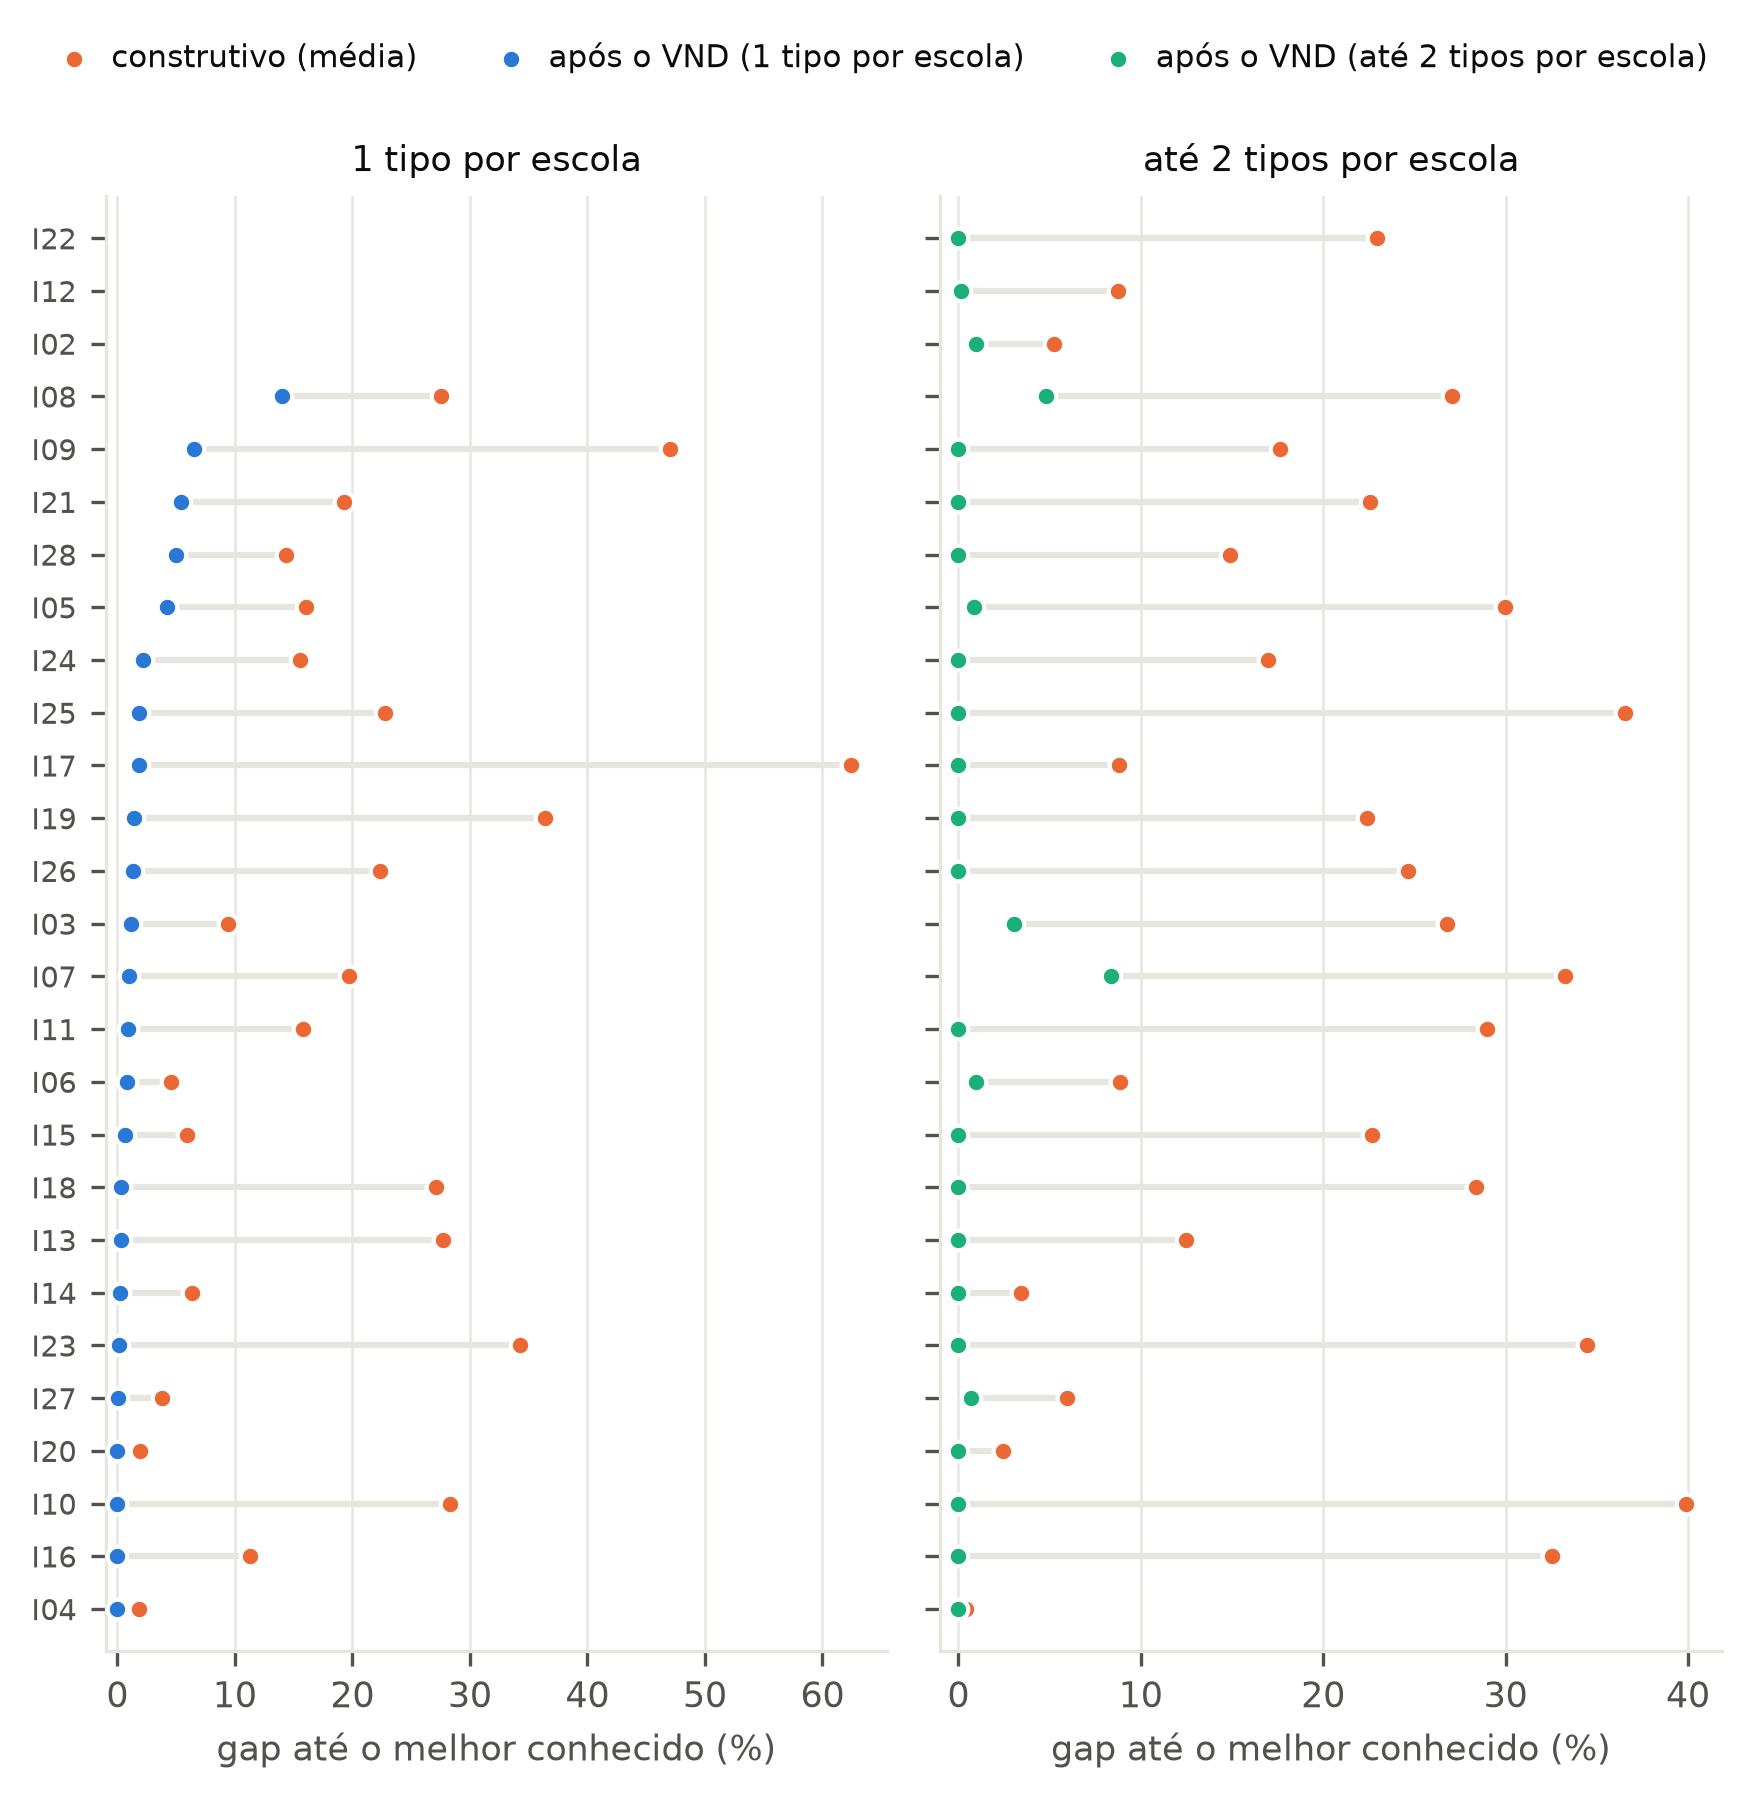
\includegraphics[width=\textwidth]{figuras/gaps.png}
  \caption{Gap até o melhor valor conhecido da solução inicial (média de 10 execuções) e da
    solução após o VND, por instância, com um e com até dois tipos por escola.}
  \label{fig:gaps}
\end{figure}

\begin{table}[htbp]
  \centering
  \caption{Um tipo por escola: valor da solução inicial (construtivo) e após o VND nas 10
    execuções (média, desvio padrão, melhor e pior).}
  \label{tab:resultados}
  \scriptsize
  \begin{tabular}{lrrrrrrrr}
\hline
 & \multicolumn{4}{c}{Construtivo (10 execuções)} & \multicolumn{4}{c}{Após o VND (10 execuções)} \\
ID & média & desvio & melhor & pior & média & desvio & melhor & pior \\
\hline
I02 & 951,64 & 0,23 & 951,35 & 952,16 & 913,13 & 0,00 & 913,13 & 913,13 \\
I03 & 1064,93 & 2,61 & 1059,85 & 1068,24 & 865,52 & 0,00 & 865,52 & 865,52 \\
I04 & 107,95 & 0,02 & 107,90 & 107,99 & 107,48 & 0,00 & 107,48 & 107,48 \\
I05 & 1291,20 & 3,58 & 1285,25 & 1297,33 & 1002,08 & 0,00 & 1002,08 & 1002,08 \\
I06 & 2014,25 & 0,96 & 2012,62 & 2015,98 & 1868,06 & 0,00 & 1868,06 & 1868,06 \\
I07 & 1454,35 & 1,50 & 1451,83 & 1456,23 & 1182,63 & 0,00 & 1182,63 & 1182,63 \\
I08 & 1207,31 & 3,99 & 1199,90 & 1215,37 & 995,56 & 0,00 & 995,56 & 995,56 \\
I09 & 19400,52 & 12,68 & 19383,59 & 19429,78 & 16495,78 & 0,00 & 16495,78 & 16495,78 \\
I10 & 35443,23 & 9,20 & 35429,92 & 35457,10 & 25340,44 & 0,00 & 25340,44 & 25340,44 \\
I11 & 7573,57 & 2,02 & 7570,62 & 7576,39 & 5870,99 & 0,00 & 5870,99 & 5870,99 \\
I12 & 705,46 & 0,01 & 705,45 & 705,47 & 649,58 & 0,00 & 649,58 & 649,58 \\
I13 & 17302,05 & 3,35 & 17297,80 & 17306,62 & 15382,63 & 0,00 & 15382,63 & 15382,63 \\
I14 & 95301,63 & 0,22 & 95301,31 & 95302,02 & 92154,42 & 0,00 & 92154,42 & 92154,42 \\
I15 & 9936,27 & 0,85 & 9935,34 & 9937,92 & 8100,75 & 0,00 & 8100,75 & 8100,75 \\
I16 & 11175,08 & 4,01 & 11170,59 & 11182,37 & 8429,94 & 0,00 & 8429,94 & 8429,94 \\
I17 & 12861,96 & 4,02 & 12854,72 & 12866,37 & 11823,63 & 0,00 & 11823,63 & 11823,63 \\
I18 & 13482,64 & 3,95 & 13476,95 & 13488,84 & 10502,73 & 0,00 & 10502,73 & 10502,73 \\
I19 & 13659,77 & 4,71 & 13654,75 & 13669,97 & 11161,55 & 0,00 & 11161,55 & 11161,55 \\
I20 & 104691,50 & 5,34 & 104683,80 & 104701,13 & 102190,57 & 0,00 & 102190,57 & 102190,57 \\
I21 & 29600,57 & 5,09 & 29591,82 & 29606,58 & 24150,26 & 0,00 & 24150,26 & 24150,26 \\
I22 & 15787,23 & 6,48 & 15778,31 & 15797,95 & 12842,92 & 0,00 & 12842,92 & 12842,92 \\
I23 & 9907,73 & 3,23 & 9902,66 & 9913,59 & 7369,43 & 0,00 & 7369,43 & 7369,43 \\
I24 & 26563,28 & 9,14 & 26547,46 & 26579,34 & 22705,46 & 0,00 & 22705,46 & 22705,46 \\
I25 & 13548,80 & 2,14 & 13544,94 & 13552,36 & 9923,36 & 0,00 & 9923,36 & 9923,36 \\
I26 & 13479,53 & 2,00 & 13474,63 & 13481,40 & 10815,79 & 0,00 & 10815,79 & 10815,79 \\
I27 & 1030,76 & 0,03 & 1030,73 & 1030,82 & 979,92 & 0,21 & 979,32 & 979,99 \\
I28 & 70848,67 & 8,85 & 70837,39 & 70869,13 & 61663,84 & 0,00 & 61663,84 & 61663,84 \\
\hline
\end{tabular}

\end{table}

\begin{table}[htbp]
  \centering
  \caption{Melhoria média da busca local, gaps da solução inicial (média) e final (melhor execução)
    até a referência, gap final até o limite inferior e tempo médio por execução ($t$), com um e
    com até dois tipos por escola. $^*$: referência com otimalidade provada.}
  \label{tab:qualidade}
  \scriptsize
  \setlength{\tabcolsep}{4pt}
  \begin{tabular}{lrrrrrrrr}
\hline
ID & Melhoria & Gap ini. & Gap final & Gap LB & $t_c$ & $t_{bl}$ & Escolas & Salas \\
 & (\%) & (\%) & (\%) & (\%) & (s) & (s) & usadas & usadas \\
\hline
I01 & 0,76 & 7,51 & 6,70$^*$ & 6,70 & 0,001 & 0,00 & 5/5 & 12/12 \\
I02 & 7,61 & 26,78 & 17,13 & 17,55 & 0,002 & 0,01 & 12/12 & 24/24 \\
I03 & 0,43 & 0,43 & 0,00$^*$ & 0,00 & 0,001 & 0,00 & 12/12 & 24/24 \\
I04 & 12,81 & 27,32 & 11,01 & 11,67 & 0,002 & 0,07 & 14/14 & 40/43 \\
I05 & 2,51 & 10,01 & 7,25$^*$ & 7,25 & 0,002 & 0,02 & 12/12 & 39/39 \\
I06 & 12,23 & 16,00 & 1,81$^*$ & 1,81 & 0,002 & 0,11 & 12/12 & 39/39 \\
I07 & 12,38 & 24,93 & 9,46$^*$ & 9,46 & 0,002 & 0,05 & 16/16 & 44/44 \\
I08 & 17,90 & 21,80 & 0,00 & 1,35 & 0,012 & 0,84 & 11/11 & 62/62 \\
I09 & 12,76 & 15,51 & 0,77 & 0,97 & 0,013 & 2,45 & 10/10 & 82/88 \\
I10 & 3,32 & 3,74 & 0,30 & 0,35 & 0,015 & 0,93 & 14/14 & 141/150 \\
I11 & 1,29 & 1,32 & 0,01$^*$ & 0,01 & 0,014 & 0,89 & 10/10 & 91/97 \\
I12 & 6,57 & 7,41 & 0,35 & 0,43 & 0,016 & 0,61 & 15/15 & 187/205 \\
I13 & 1,81 & 1,85 & 0,01 & 0,02 & 0,018 & 0,52 & 15/15 & 180/205 \\
I14 & 11,52 & 13,46 & 0,39 & 0,45 & 0,016 & 2,30 & 12/12 & 123/142 \\
I15 & 9,18 & 10,35 & 0,22 & 0,26 & 0,015 & 1,60 & 12/12 & 129/145 \\
I16 & 7,93 & 9,16 & 0,51 & 0,63 & 0,017 & 0,79 & 14/14 & 148/150 \\
I17 & 11,75 & 13,35 & 0,03 & 1,29 & 0,016 & 2,15 & 15/15 & 115/117 \\
I18 & 6,47 & 7,29 & 0,35 & 0,50 & 0,018 & 1,42 & 15/15 & 146/157 \\
I19 & 2,51 & 2,57 & 0,00 & 0,01 & 0,022 & 4,23 & 13/15 & 101/122 \\
I20 & 18,66 & 23,91 & 0,79 & 1,05 & 0,021 & 1,83 & 15/15 & 121/125 \\
I21 & 17,44 & 21,12 & 0,00 & 0,20 & 0,022 & 7,23 & 15/15 & 120/125 \\
I22 & 13,03 & 14,98 & 0,00 & 1,76 & 0,017 & 2,93 & 15/15 & 101/101 \\
I23 & 6,72 & 7,21 & 0,00 & 0,16 & 0,020 & 10,38 & 15/15 & 175/177 \\
I24 & 15,69 & 18,60 & 0,00 & 4,07 & 0,020 & 0,44 & 15/15 & 101/101 \\
I25 & 11,01 & 12,37 & 0,00 & 0,44 & 0,021 & 40,72 & 15/15 & 241/248 \\
I26 & 3,77 & 4,00 & 0,08$^*$ & 0,08 & 0,024 & 2,19 & 20/20 & 190/197 \\
I27 & 8,18 & 8,90 & 0,00 & 0,62 & 0,036 & 0,63 & 20/20 & 112/113 \\
\hline
\end{tabular}

\end{table}

\subsection{Contribuição de cada vizinhança}

A Tabela~\ref{tab:vizinhancas} e a Figura~\ref{fig:vizinhancas} mostram quanto cada vizinhança
contribui. A N2 (swap) responde pela maior parte da melhoria nos dois casos
(\partNDoisUm\% com $K = 1$ e \partNDoisDois\% com $K = 2$), o que confirma a escolha motivada pela
folga pequena: com as escolas cheias, o ganho vem de trocar candidatos. A N1 quase não atua logo
após o construtivo, pois a fase B já coloca cada candidato na escola mais próxima com vaga; ela volta
a ser útil depois das mudanças de tipo, que abrem vagas novas. A N3 tem contribuição pequena em
valor, mas é ela que garante que a alocação final é ótima para os tipos encontrados.

As vizinhanças de tipos se comportam de forma muito diferente nos dois casos, como previsto ao
projetá-las. Com $K = 1$, N4 e N5 não atuam (todas as escolas têm mais de uma sala, e só há um tipo
por escola), N6 atua pouco (\partNSeisUm\%), porque a cobertura justa raramente permite que uma
escola inteira mude de tipo sozinha, e \textbf{N7 é a segunda vizinhança mais importante}
(\partNSeteUm\% da melhoria): trocar os tipos de duas escolas mantém a cobertura quase intacta. Com
$K = 2$, a escola tem duas partes ajustáveis e N4 passa a ser a segunda mais importante
(\partNQuatroDois\%), seguida de N7 (\partNSeteDois\%).

\begin{table}[htbp]
  \centering
  \caption{Movimentos aplicados por execução, ganho por execução (em \% do valor inicial) e
    participação de cada vizinhança na melhoria total (médias por instância), com um e com até
    dois tipos por escola.}
  \label{tab:vizinhancas}
  \small
  \begin{tabular}{lrrr}
\hline
Vizinhança & Movimentos & Ganho & \% da melhoria \\
\hline
N1 shift & 177,7 & 0,83\% & 4,8 \\
N2 swap & 1627,9 & 8,62\% & 57,2 \\
N3 cadeias & 204,2 & 0,49\% & 3,1 \\
N4 retipar sala & 19,8 & 3,02\% & 18,0 \\
N5 trocar salas & 21,8 & 0,40\% & 2,6 \\
N6 tipo da escola & 1,9 & 0,63\% & 4,4 \\
N7 trocar escolas & 3,6 & 1,30\% & 10,0 \\
\hline
\end{tabular}

\end{table}

\begin{figure}[htbp]
  \centering
  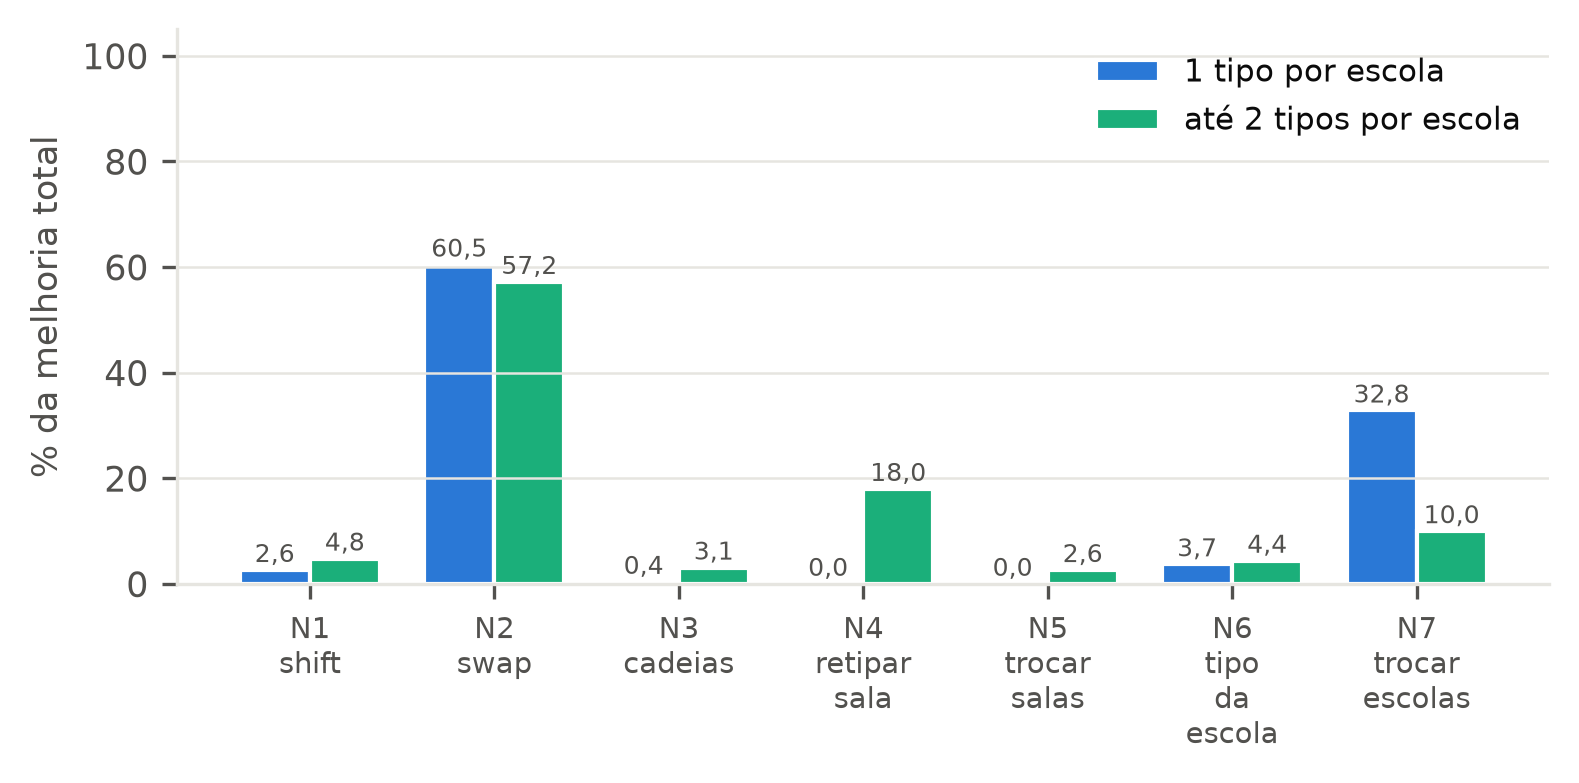
\includegraphics[width=\textwidth]{figuras/vizinhancas.png}
  \caption{Participação de cada vizinhança na melhoria obtida pelo VND, com um e com até dois tipos
    por escola.}
  \label{fig:vizinhancas}
\end{figure}

\subsection{Tempo de execução}

O construtivo leva no máximo \tConstrMaxUm~s com $K = 1$ e \tConstrMaxDois~s com
$K = 2$ (incluindo o reparo exato, quando usado). O tempo total (Figura~\ref{fig:tempo}) é dominado
pelo VND: com $K = 1$, \tempoMedioUm~s em média e \tempoMaxUm~s no caso mais lento
(\tempoMaxIdUm); com $K = 2$, \tempoMedioDois~s em média e \tempoMaxDois~s no máximo
(\tempoMaxIdDois). O tempo cresce com o número de candidatos (correlação de \corrTempoMUm{} e
\corrTempoMDois{} entre o tempo da busca e $M$, por execução), mas acompanha ainda mais o número de
mudanças de tipo aceitas em N4 a N7 (\corrTempoTiposUm{} e \corrTempoTiposDois), porque cada
mudança aceita reinicia a VND em N1, que volta a percorrer todos os candidatos. Com $K = 2$ há mais
mudanças de tipo possíveis e aceitas, o que explica o tempo cinco vezes maior.

\begin{figure}[htbp]
  \centering
  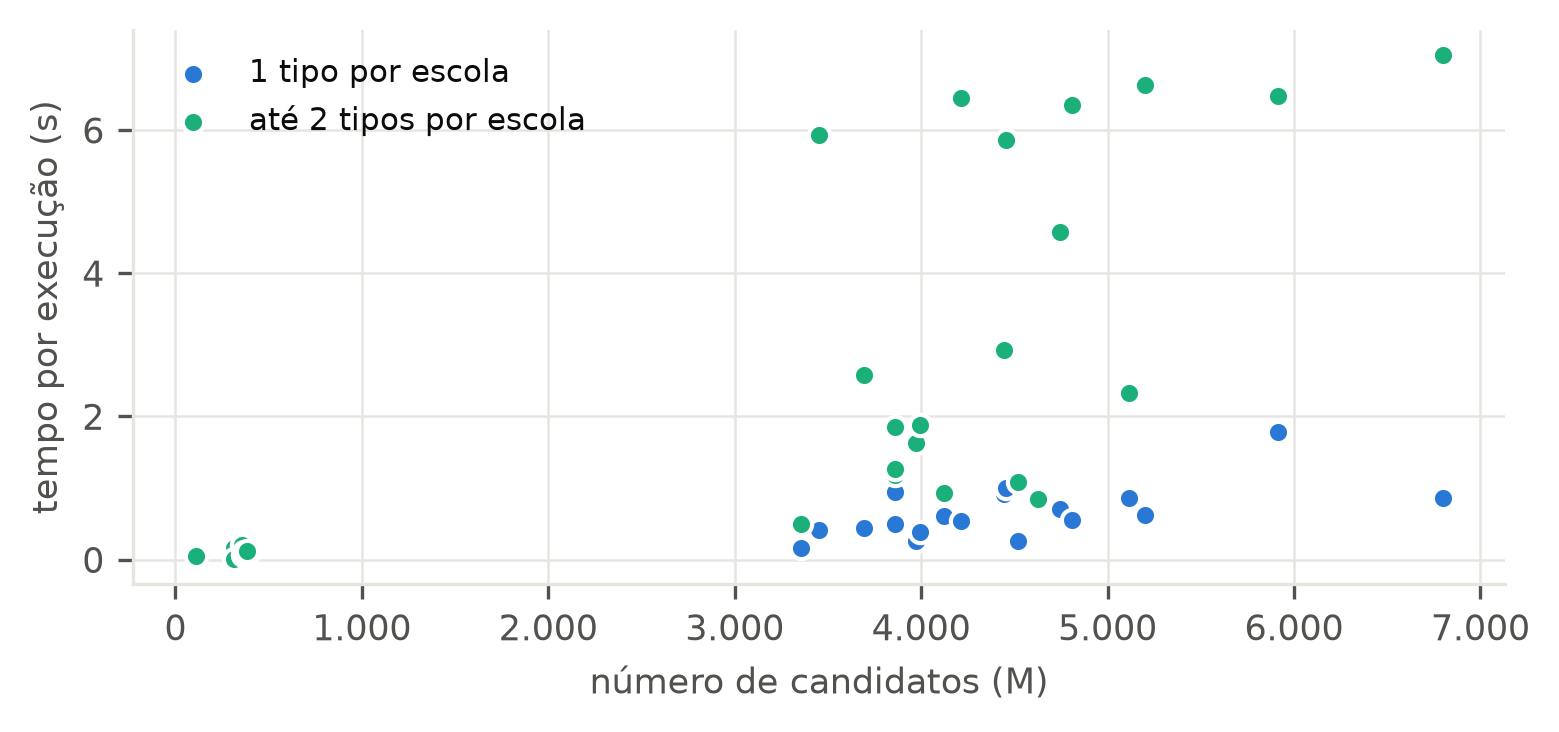
\includegraphics[width=\textwidth]{figuras/tempo.png}
  \caption{Tempo médio por execução (construtivo e VND) em função do número de candidatos.}
  \label{fig:tempo}
\end{figure}

\subsection{Variabilidade}

A Figura~\ref{fig:variabilidade} mostra o desvio de cada execução em relação à média da
instância. O construtivo varia pouco (coeficiente de variação médio de \cvIniUm\% com $K = 1$,
máximo de \cvIniMaxUm\%), e o VND termina \textbf{no mesmo valor} nas 10 execuções de todas as
instâncias com $K = 1$; com $K = 2$, só \nVariaFinDois{} instância tem alguma variação no valor final
(CV de \cvFinMaxDois\%). Isso indica que a aleatoriedade da fase B altera apenas a ordem de
candidatos com arrependimentos parecidos, e o VND corrige essas diferenças, porque os tipos (a
decisão que de fato define o ótimo local) vêm da fase A, que é determinística. O resultado final é,
portanto, robusto à semente; em contrapartida, a RCL da fase B não gera diversidade suficiente para
escapar do ótimo local, o que motiva as melhorias da Seção~\ref{sec:conclusao}.

\begin{figure}[htbp]
  \centering
  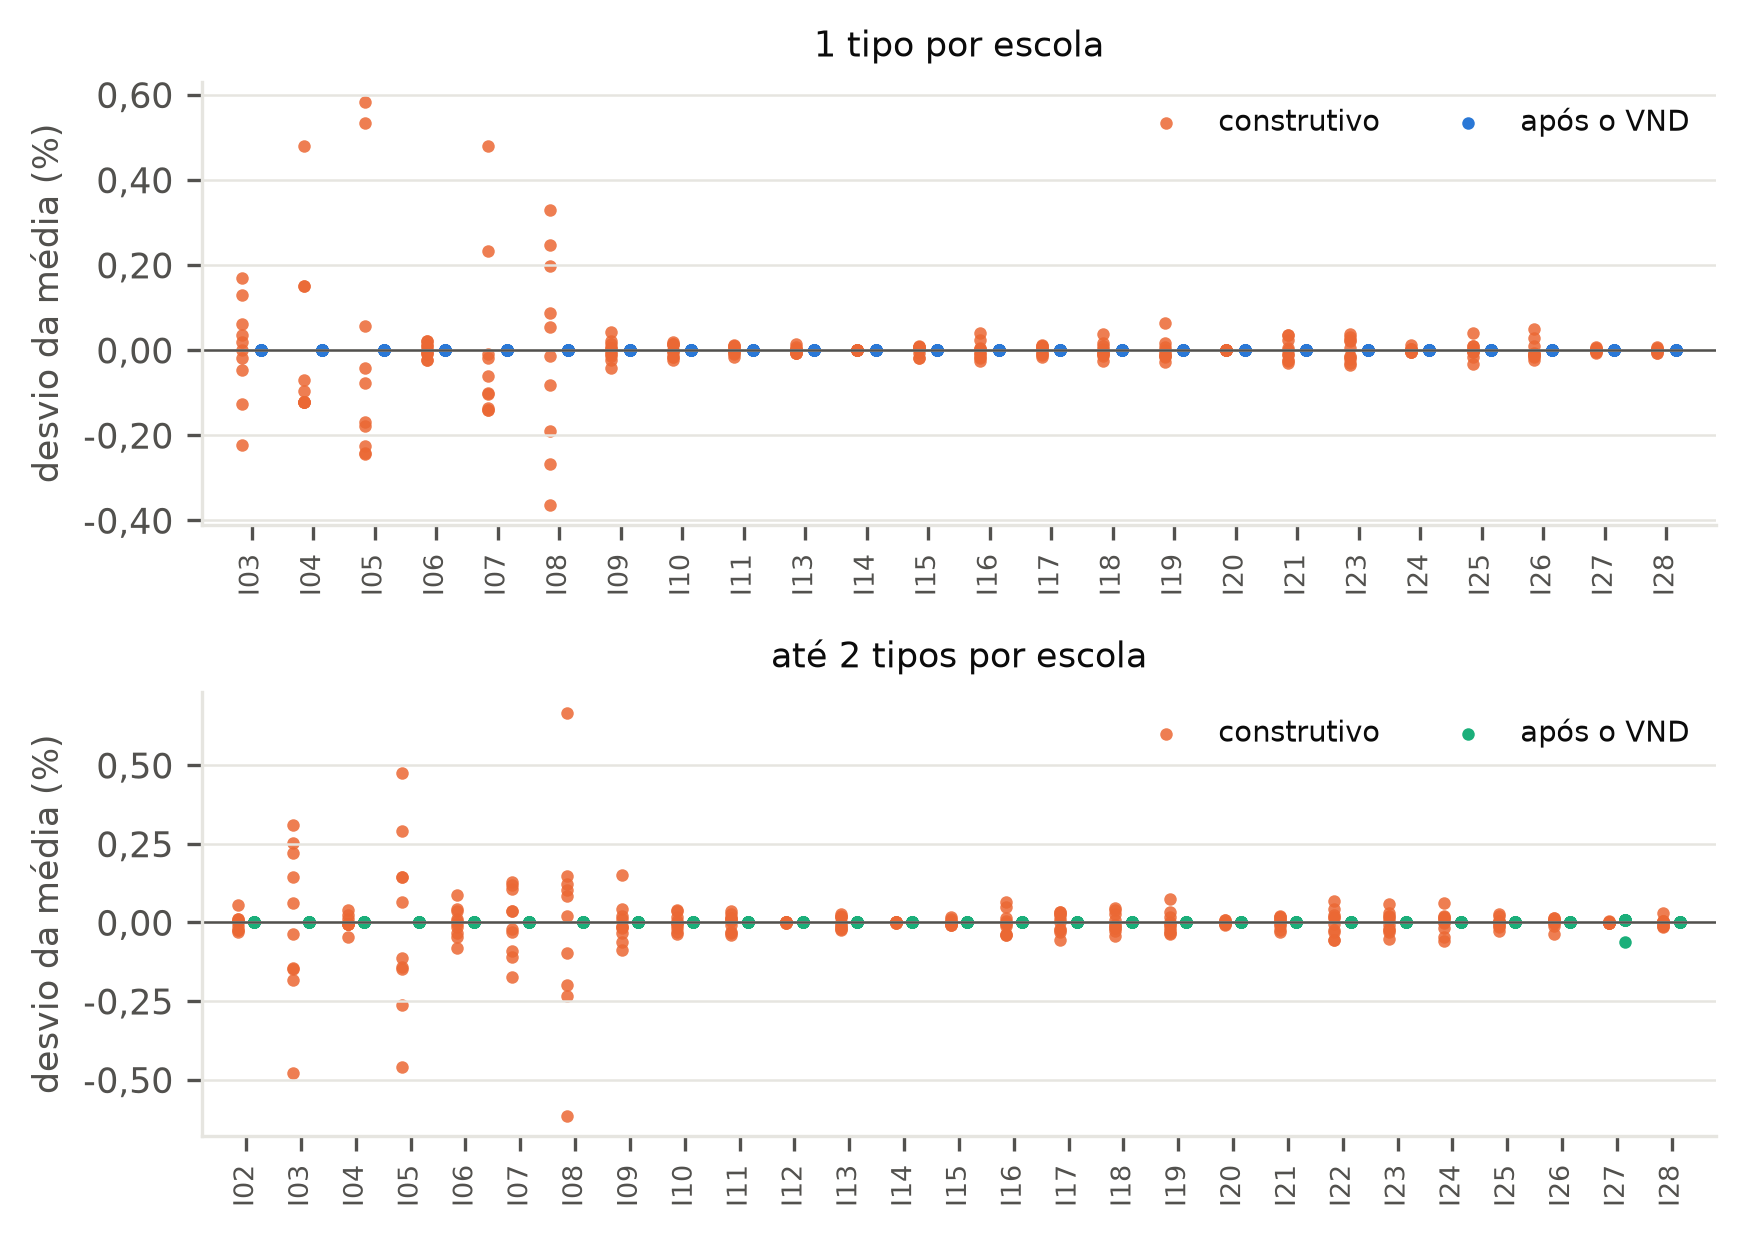
\includegraphics[width=\textwidth]{figuras/variabilidade.png}
  \caption{Desvio percentual de cada uma das 10 execuções em relação à média da instância, na
    solução inicial e após o VND.}
  \label{fig:variabilidade}
\end{figure}

\subsection{Sensibilidade ao tamanho da RCL}\label{sec:sensibilidade}

Para escolher o tamanho da RCL, repetimos o experimento com $K = 1$ para $k \in \{1, 5, 25, 50\}$
(com $k = 1$, uma única execução, pois o construtivo é determinístico). A
Tabela~\ref{tab:sensibilidade} mostra a média, sobre as instâncias, do gap da solução
inicial e da final e do coeficiente de variação (CV) entre as 10 execuções.

\begin{table}[htbp]
  \centering
  \caption{Sensibilidade ao tamanho da RCL ($K = 1$): gaps médios e coeficiente de variação
    médio entre execuções.}
  \label{tab:sensibilidade}
  \scriptsize
  \begin{tabular}{rrrrrrr}
\hline
$k$ & Gap ini. (\%) & Gap final (\%) & Gap final melhor (\%) & CV ini. (\%) & CV final (\%) & $t$ (s) \\
\hline
1 & 19,97 & 0,735 & 0,735 & 0,000 & 0,000 & 2,62 \\
5 & 19,96 & 0,735 & 0,735 & 0,048 & 0,000 & 2,58 \\
10 & 19,96 & 0,734 & 0,732 & 0,056 & 0,001 & 2,56 \\
25 & 19,96 & 0,733 & 0,732 & 0,109 & 0,001 & 2,58 \\
50 & 20,00 & 0,734 & 0,732 & 0,129 & 0,001 & 2,58 \\
\hline
\end{tabular}

\end{table}

Aumentar $k$ aumenta a dispersão do construtivo e piora ligeiramente a solução inicial média,
como esperado ao sortear entre candidatos com arrependimento menor. Mas \textbf{o valor final é
idêntico para todo $k$}: o VND converge para o mesmo ótimo local, e o tempo não muda. Mantivemos
$k = 10$ como padrão porque gera variação mensurável entre execuções sem degradar a solução inicial.
O experimento mostra, porém, que a diversidade necessária para melhorar o resultado final não virá
da RCL da fase B, e sim de perturbações nos tipos das escolas (Seção~\ref{sec:conclusao}).

\subsection{Informações da solução: locais utilizados e distribuição}

Como não há custo de abertura e a folga é pequena, todas as escolas são usadas em todas as
instâncias com $K = 1$; com $K = 2$, só uma instância (I20, a de maior folga) deixa uma escola
fechada (Tabela~\ref{tab:tipos-por-escola}). A Figura~\ref{fig:distribuicao} e a
Tabela~\ref{tab:distribuicao} mostram a distribuição dos candidatos na melhor solução da instância
do grupo \idGrupo{} (5917 candidatos, 20 escolas, 197 salas). Com $K = 1$, cada tipo fica com três
ou quatro escolas, e a folga se concentra nas escolas do tipo com mais sobra (E1, M3d, usa só 52\%
da capacidade). Com $K = 2$ todas as 20 escolas oferecem dois tipos, cada tipo aparece em seis a
oito escolas, e quase todas as escolas ficam cheias; ainda assim a distância total cai só
\reducaoGrupo\%, porque nessa instância a solução com um tipo já fica perto do LB
(Tabela~\ref{tab:tipos-por-escola}).

\begin{figure}[htbp]
  \centering
  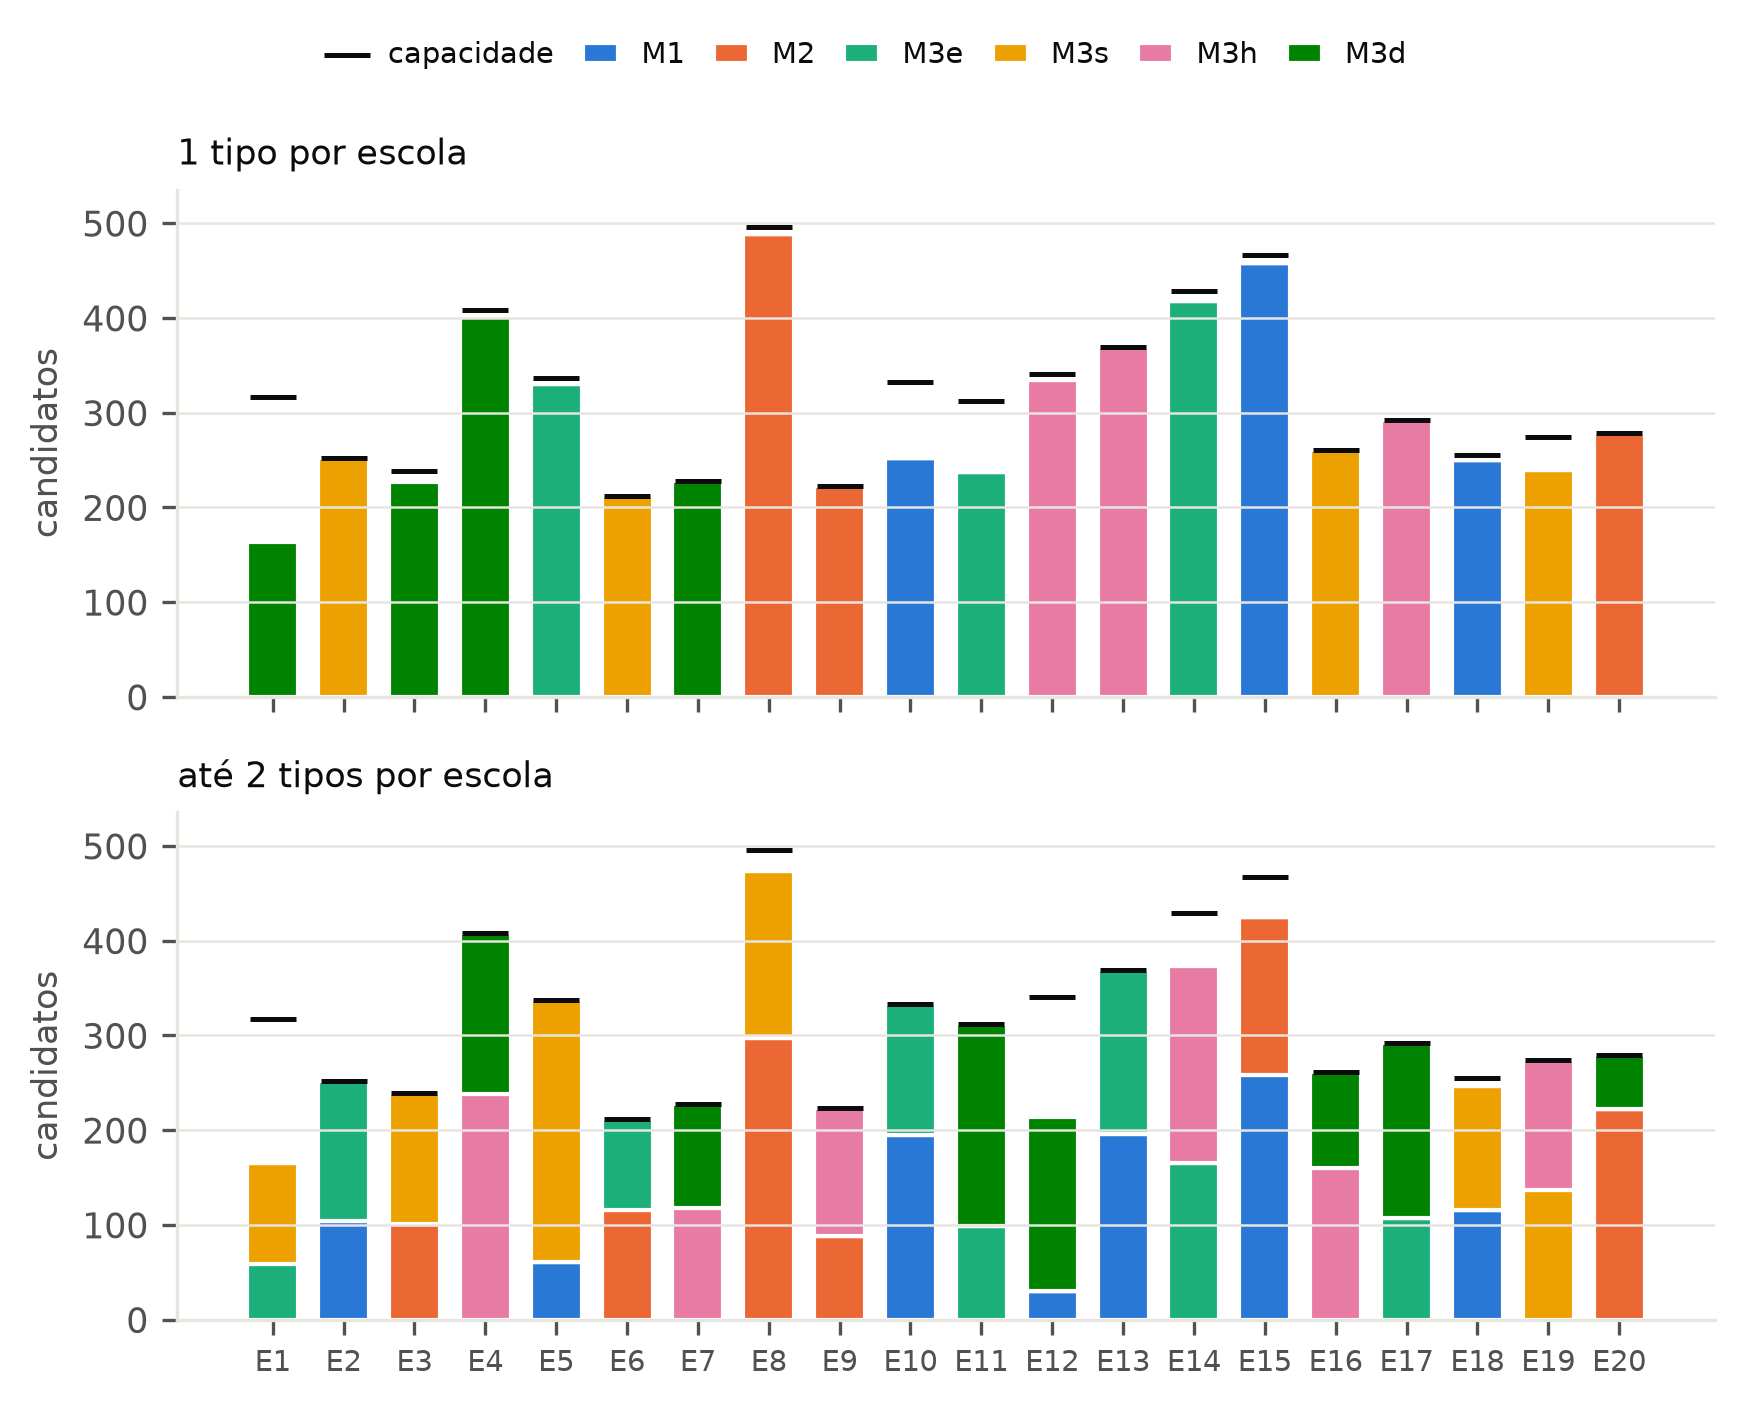
\includegraphics[width=\textwidth]{figuras/distribuicao.png}
  \caption{Candidatos por escola e tipo de prova na melhor solução de \idGrupo{}, com um e com até
    dois tipos por escola; o traço preto indica a capacidade da escola.}
  \label{fig:distribuicao}
\end{figure}

\begin{table}[htbp]
  \centering
  \caption{Resumo por escola da melhor solução de \idGrupo{}: capacidade, tipos oferecidos,
    candidatos, ocupação e distância média, com um e com até dois tipos por escola.}
  \label{tab:distribuicao}
  \scriptsize
  \setlength{\tabcolsep}{4pt}
  \begin{tabular}{lrrrrrr}
\hline
Escola & Salas usadas & Tipos & Capacidade & Candidatos & Ocupação (\%) & Dist. média \\
\hline
E1 & 5/5 & 5 & 317 & 297 & 93,7 & 0,212 \\
E2 & 13/13 & 6 & 252 & 252 & 100,0 & 0,002 \\
E3 & 11/11 & 6 & 239 & 239 & 100,0 & 0,129 \\
E4 & 15/15 & 6 & 408 & 408 & 100,0 & 0,053 \\
E5 & 8/8 & 6 & 337 & 337 & 100,0 & 0,073 \\
E6 & 11/11 & 6 & 212 & 212 & 100,0 & 0,009 \\
E7 & 5/5 & 5 & 228 & 228 & 100,0 & 0,086 \\
E8 & 11/11 & 6 & 496 & 483 & 97,4 & 0,080 \\
E9 & 11/11 & 6 & 223 & 223 & 100,0 & 0,033 \\
E10 & 12/12 & 6 & 333 & 333 & 100,0 & 0,775 \\
E11 & 14/14 & 6 & 312 & 312 & 100,0 & 0,116 \\
E12 & 10/10 & 6 & 341 & 341 & 100,0 & 0,245 \\
E13 & 12/12 & 6 & 369 & 369 & 100,0 & 0,224 \\
E14 & 11/12 & 6 & 429 & 336 & 78,3 & 0,251 \\
E15 & 8/8 & 5 & 467 & 428 & 91,6 & 0,022 \\
E16 & 5/5 & 5 & 261 & 261 & 100,0 & 0,355 \\
E17 & 8/9 & 5 & 292 & 260 & 89,0 & 0,011 \\
E18 & 3/7 & 3 & 255 & 67 & 26,3 & 0,198 \\
E19 & 7/8 & 6 & 274 & 252 & 92,0 & 0,014 \\
E20 & 10/10 & 6 & 279 & 279 & 100,0 & 0,310 \\
\hline
\end{tabular}

\end{table}

\subsection{Um contra dois tipos por escola}\label{sec:tipos-por-escola}

Repetimos o experimento principal (10 execuções por instância, $k = 10$) com até dois
tipos por escola (\texttt{-{}-tipos-por-escola 2}), num total de \nExecDois{} execuções. A
Tabela~\ref{tab:tipos-por-escola} compara as melhores soluções, a Figura~\ref{fig:tipos-por-escola}
mostra o gap até o limite inferior de transporte (o único que vale para os dois valores de $K$) e a
Tabela~\ref{tab:resultados-tipos2} traz os valores das 10 execuções.

\begin{itemize}
  \item \textbf{Viabilidade.} Com $K = 2$, \nInstDois{} instâncias têm solução, contra \nInstUm{}
    com $K = 1$: \soDois{} passam a ser viáveis, pois dois tipos por escola dobram o número de
    ``vagas de tipo'' (com \soDoisNmin{} escolas, por exemplo, $K = 1$ não consegue sequer
    oferecer os seis tipos).
  \item \textbf{Distância.} Em nenhuma instância a melhor solução com $K = 2$ fica pior que a com
    $K = 1$ (o que é esperado, pois é uma relaxação). A distância total cai \reducao\% em média,
    de \reducaoMin\% (\reducaoMinId) a \reducaoMax\% (\reducaoMaxId), e cai pelo menos 5\% em
    \nReducaoCinco{} das \nComp{} instâncias. O gap médio até o LB de transporte vai de
    \gapTranspUm\% para \gapTranspDois\%: o segundo tipo elimina, em média, \fechado\% da distância
    entre a solução com um tipo e o LB.
  \item \textbf{Por quê.} Com um tipo por escola, cada tipo fica, em média, com $N/6$ escolas, e
    muitos candidatos viajam longe apenas para encontrar uma escola do seu tipo. Com dois, cada tipo
    fica com cerca de $N/3$ escolas, e a escola mais próxima atende o tipo do candidato com
    frequência muito maior. O ganho é pequeno onde a solução com um tipo já ficava perto do LB
    (\reducaoMinId, I14 e \idGrupo, com gaps abaixo de 7\%).
  \item \textbf{Uso do segundo tipo.} Na melhor solução, \duasMedia\% das escolas oferecem dois
    tipos, em média (de \duasMin\% a \duasMax\% por instância). O modelo não atribui custo a abrir
    um segundo tipo numa escola, então a heurística o faz sempre que isso reduz a distância. Se um
    segundo tipo tiver custo na prática (mais coordenadores, mais malotes de provas), o natural é
    acrescentar à função objetivo uma penalidade por escola com dois tipos.
  \item \textbf{Tempo.} O tempo médio por execução vai de \tempoMedioUm~s para \tempoMedioDois~s
    (Figura~\ref{fig:tempo}), pois há mais movimentos de tipo possíveis.
\end{itemize}

\begin{figure}[htbp]
  \centering
  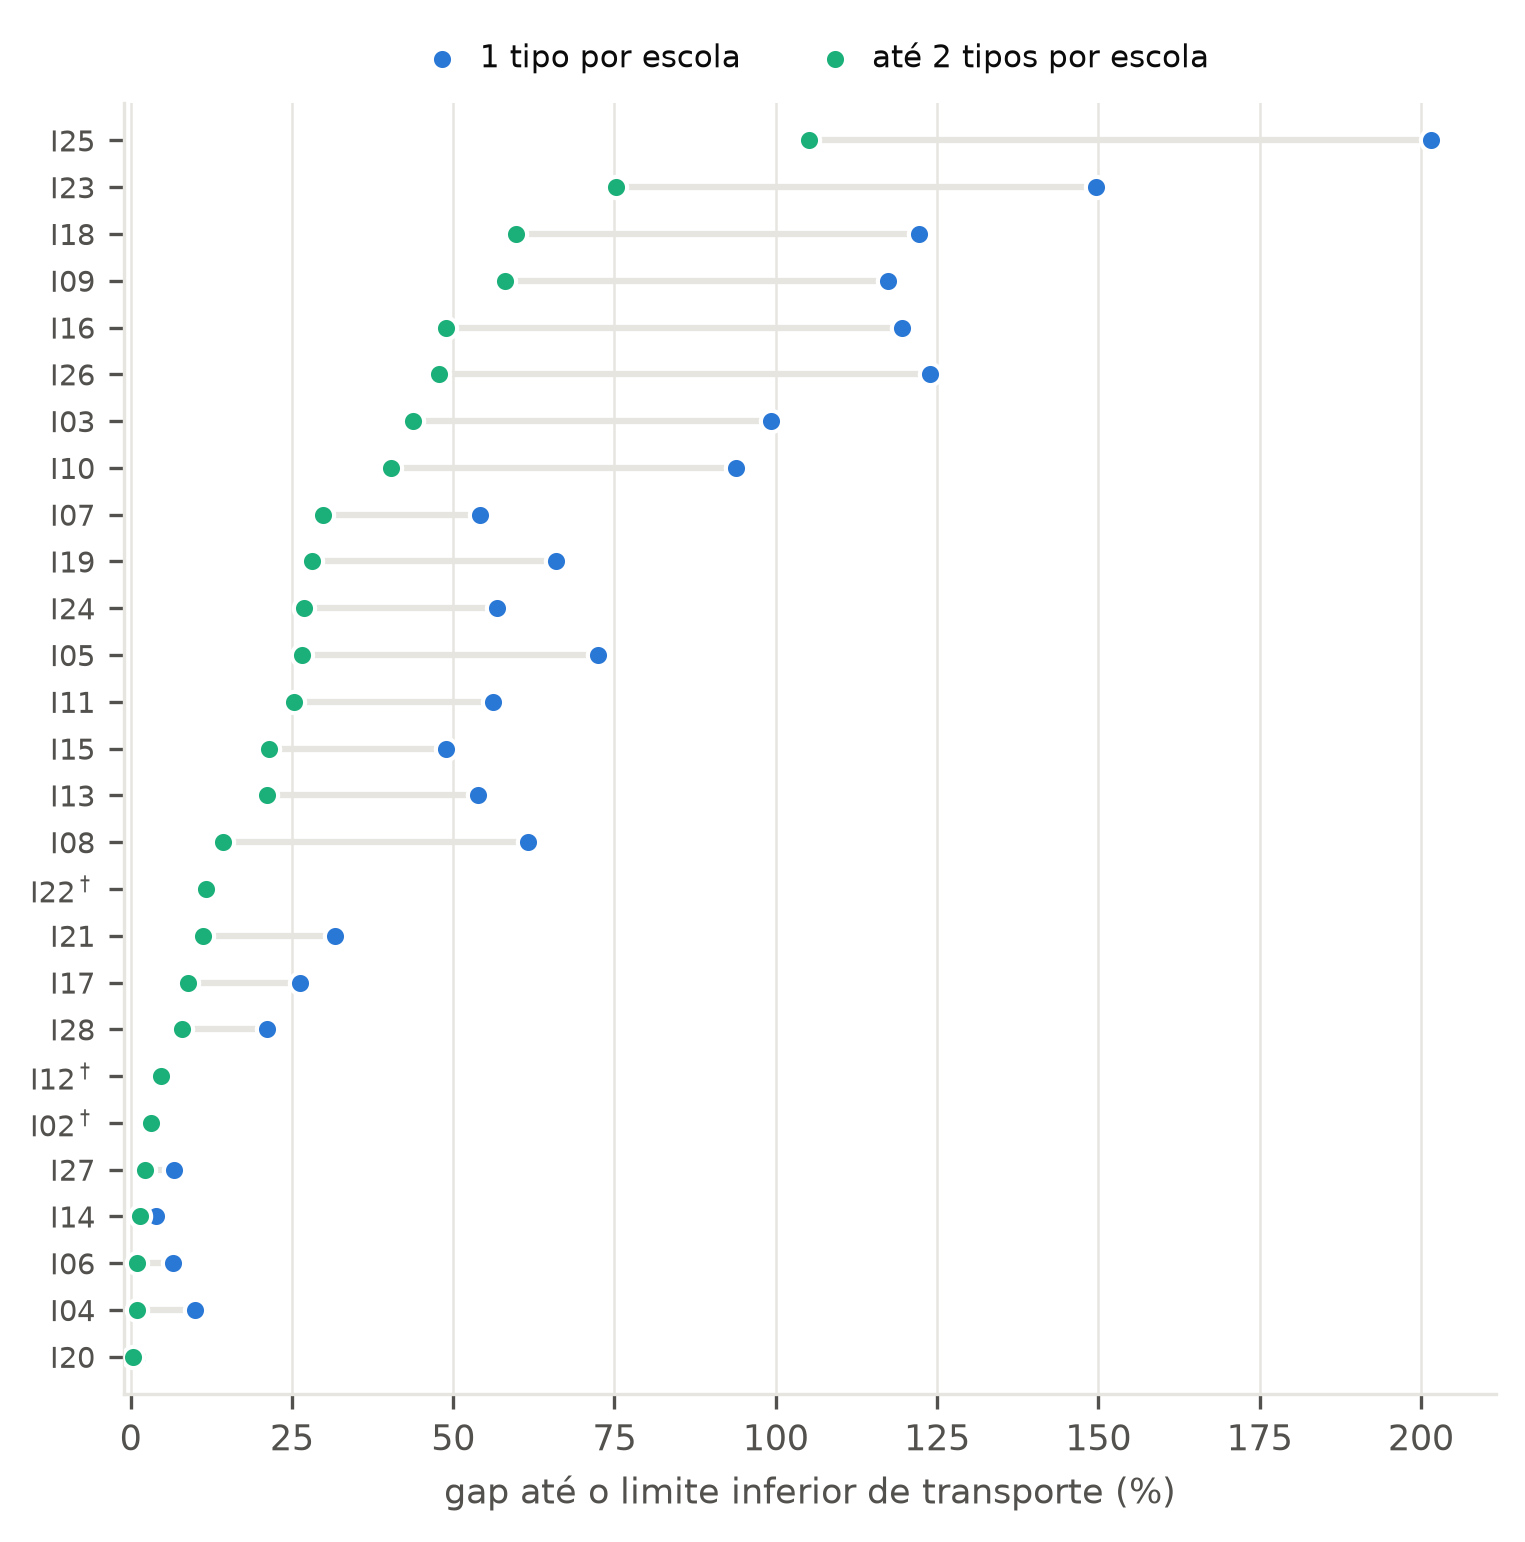
\includegraphics[width=\textwidth]{figuras/tipos_por_escola.png}
  \caption{Gap até o limite inferior de transporte da melhor solução com um e com até dois tipos
    por escola. $^\dagger$: inviável com um tipo por escola.}
  \label{fig:tipos-por-escola}
\end{figure}

\begin{table}[htbp]
  \centering
  \caption{Comparação entre um e até dois tipos por escola: melhor valor das 10 execuções, redução
    da distância, gap até o limite inferior de transporte, escolas que oferecem dois tipos e
    escolas usadas na melhor solução com até dois tipos.}
  \label{tab:tipos-por-escola}
  \scriptsize
  \begin{tabular}{lrrrrrcc}
\hline
 & \multicolumn{2}{c}{Melhor valor} & Redução & \multicolumn{2}{c}{Gap até o LB (\%)} & Escolas com & Escolas \\
ID & 1 tipo & 2 tipos & (\%) & 1 tipo & 2 tipos & 2 tipos & usadas \\
\hline
I02 & inviável & 913,13 & -- & -- & 3,08 & 5/5 & 5/5 \\
I03 & 1198,95 & 865,52 & 27,81 & 99,26 & 43,85 & 11/12 & 12/12 \\
I04 & 117,08 & 107,48 & 8,20 & 9,97 & 0,95 & 6/12 & 12/12 \\
I05 & 1366,23 & 1002,08 & 26,65 & 72,46 & 26,49 & 14/14 & 14/14 \\
I06 & 1969,52 & 1868,06 & 5,15 & 6,55 & 1,06 & 7/12 & 12/12 \\
I07 & 1404,36 & 1182,63 & 15,79 & 54,16 & 29,82 & 12/12 & 12/12 \\
I08 & 1407,00 & 995,56 & 29,24 & 61,55 & 14,31 & 15/16 & 16/16 \\
I09 & 22680,78 & 16495,78 & 27,27 & 117,35 & 58,08 & 11/11 & 11/11 \\
I10 & 34967,19 & 25340,44 & 27,53 & 93,79 & 40,44 & 10/10 & 10/10 \\
I11 & 7315,24 & 5870,99 & 19,74 & 56,12 & 25,29 & 14/14 & 14/14 \\
I12 & inviável & 649,58 & -- & -- & 4,66 & 10/10 & 10/10 \\
I13 & 19535,23 & 15382,63 & 21,26 & 53,86 & 21,15 & 15/15 & 15/15 \\
I14 & 94458,99 & 92154,42 & 2,44 & 3,93 & 1,40 & 15/15 & 15/15 \\
I15 & 9931,68 & 8100,75 & 18,44 & 48,96 & 21,50 & 12/12 & 12/12 \\
I16 & 12426,61 & 8429,94 & 32,16 & 119,56 & 48,94 & 12/12 & 12/12 \\
I17 & 13704,53 & 11823,63 & 13,72 & 26,21 & 8,89 & 14/14 & 14/14 \\
I18 & 14598,64 & 10502,73 & 28,06 & 122,13 & 59,81 & 15/15 & 15/15 \\
I19 & 14466,18 & 11161,55 & 22,84 & 66,00 & 28,08 & 15/15 & 15/15 \\
I20 & 102814,54 & 102190,57 & 0,61 & 0,98 & 0,37 & 14/15 & 14/15 \\
I21 & 28595,46 & 24150,26 & 15,55 & 31,74 & 11,26 & 15/15 & 15/15 \\
I22 & inviável & 12842,92 & -- & -- & 11,72 & 15/15 & 15/15 \\
I23 & 10497,91 & 7369,43 & 29,80 & 149,68 & 75,27 & 15/15 & 15/15 \\
I24 & 28047,77 & 22705,46 & 19,05 & 56,77 & 26,91 & 15/15 & 15/15 \\
I25 & 14586,95 & 9923,36 & 31,97 & 201,56 & 105,15 & 14/15 & 15/15 \\
I26 & 16389,12 & 10815,79 & 34,01 & 123,96 & 47,80 & 15/15 & 15/15 \\
I27 & 1021,42 & 979,32 & 4,12 & 6,69 & 2,29 & 20/20 & 20/20 \\
I28 & 69185,46 & 61663,84 & 10,87 & 21,10 & 7,93 & 20/20 & 20/20 \\
\hline
\end{tabular}

\end{table}

\begin{table}[htbp]
  \centering
  \caption{Até dois tipos por escola: valor da solução inicial e após o VND nas 10 execuções (média,
    desvio padrão, melhor e pior).}
  \label{tab:resultados-tipos2}
  \scriptsize
  \begin{tabular}{lrrrrrrrr}
\hline
 & \multicolumn{4}{c}{Construtivo (10 execuções)} & \multicolumn{4}{c}{Após o VND (10 execuções)} \\
ID & média & desvio & melhor & pior & média & desvio & melhor & pior \\
\hline
I01 & 893,82 & 0,59 & 892,69 & 894,68 & 890,82 & 0,00 & 890,82 & 890,82 \\
I02 & 829,15 & 2,52 & 824,53 & 831,80 & 690,75 & 0,00 & 690,75 & 690,75 \\
I03 & 106,47 & 0,01 & 106,47 & 106,48 & 106,47 & 0,00 & 106,47 & 106,47 \\
I04 & 944,09 & 4,05 & 937,01 & 951,05 & 852,41 & 0,00 & 852,41 & 852,41 \\
I05 & 2010,59 & 1,35 & 2008,83 & 2013,04 & 1926,53 & 0,00 & 1926,53 & 1926,53 \\
I06 & 1066,86 & 4,13 & 1056,37 & 1069,93 & 935,11 & 0,00 & 935,11 & 935,11 \\
I07 & 1018,53 & 4,19 & 1013,42 & 1026,14 & 901,12 & 0,00 & 901,12 & 901,12 \\
I08 & 10931,57 & 8,36 & 10918,61 & 10943,23 & 10469,72 & 0,00 & 10469,72 & 10469,72 \\
I09 & 20860,35 & 10,27 & 20846,65 & 20880,20 & 18154,99 & 0,00 & 18154,99 & 18154,99 \\
I10 & 4851,70 & 0,70 & 4850,14 & 4852,66 & 4706,56 & 0,00 & 4706,56 & 4706,56 \\
I11 & 620,86 & 0,00 & 620,86 & 620,86 & 620,69 & 0,00 & 620,69 & 620,69 \\
I12 & 13524,85 & 3,36 & 13519,05 & 13529,16 & 12712,86 & 0,00 & 12712,86 & 12712,86 \\
I13 & 92533,81 & 0,60 & 92532,89 & 92534,78 & 90895,96 & 0,00 & 90895,96 & 90895,96 \\
I14 & 7530,10 & 2,33 & 7525,60 & 7532,74 & 6682,65 & 0,00 & 6682,65 & 6682,65 \\
I15 & 6216,37 & 2,68 & 6212,14 & 6221,09 & 5669,53 & 0,00 & 5669,53 & 5669,53 \\
I16 & 11918,66 & 3,19 & 11913,06 & 11923,76 & 10903,04 & 0,00 & 10903,04 & 10903,04 \\
I17 & 7486,50 & 4,17 & 7479,28 & 7492,22 & 6611,84 & 0,00 & 6611,84 & 6611,84 \\
I18 & 9246,47 & 3,92 & 9237,05 & 9250,99 & 8735,08 & 0,00 & 8735,08 & 8735,08 \\
I19 & 104382,37 & 2,21 & 104378,71 & 104385,49 & 101824,03 & 0,00 & 101824,03 & 101824,03 \\
I20 & 26750,82 & 5,97 & 26739,73 & 26761,64 & 21820,85 & 0,00 & 21820,85 & 21820,85 \\
I21 & 13870,39 & 6,90 & 13859,46 & 13878,50 & 11511,41 & 0,00 & 11511,41 & 11511,41 \\
I22 & 4627,91 & 2,25 & 4624,62 & 4630,79 & 4223,82 & 0,00 & 4223,82 & 4223,82 \\
I23 & 19197,53 & 3,07 & 19194,02 & 19202,71 & 17906,74 & 0,00 & 17906,74 & 17906,74 \\
I24 & 5733,40 & 2,42 & 5731,15 & 5737,61 & 4971,06 & 0,00 & 4971,06 & 4971,06 \\
I25 & 7751,56 & 3,42 & 7746,24 & 7756,53 & 7329,36 & 0,00 & 7329,36 & 7329,36 \\
I26 & 994,25 & 0,01 & 994,22 & 994,26 & 958,16 & 0,00 & 958,16 & 958,16 \\
I27 & 62297,48 & 10,33 & 62281,74 & 62316,51 & 57295,51 & 0,00 & 57295,51 & 57295,51 \\
I28 & 856,36 & 1,43 & 854,31 & 858,32 & 841,58 & 0,00 & 841,58 & 841,58 \\
\hline
\end{tabular}

\end{table}

% =====================================================================================
\section{Exemplo passo a passo}\label{sec:exemplo}

Usamos a instância \idExemplo{} (316 candidatos, 12 escolas com duas salas cada, de 15 e
16 lugares, ou seja, 31 lugares por escola; 53 candidatos de cada tipo M1 a M3s e 52 de M3h e M3d),
com semente 0 e $k = 10$. O registro completo é gerado pela opção \texttt{-{}-traco} do programa.

\textbf{Fase A ($K = 1$).} A alocação provisória estima, por exemplo, para a escola E1:
M1 = 5, M2 = 6, M3e = 8, M3s = 3, M3h = 3, M3d = 4. Com um tipo por escola, E1 fica com M3e, o de
maior demanda estimada, e as suas duas salas recebem M3e. Repetindo para as 12 escolas, M1, M2, M3e
e M3h ficam com duas escolas cada (62 vagas), M3s com três (93 vagas) e M3d com apenas uma (31 vagas
para 52 candidatos). A etapa de cobertura muda E7 inteira de M3s para M3d, o que é possível porque
M3s continua com 62 vagas para 53 candidatos. Ao final, cada tipo tem 62 vagas.

\textbf{Fase B.} Os 10 candidatos de maior arrependimento formam a RCL (C213, C294, C172, \ldots,
com arrependimentos de 4,03 a 3,65). O sorteio escolhe C287 (tipo M3s); as sete escolas mais
próximas dele não oferecem M3s, e ele vai para E4, sala 1. C287 sai da RCL e entra C290, o 11º da
fila. O processo segue até os 316 candidatos estarem alocados, com custo inicial de 1297,64.

\textbf{VND ($K = 1$).} N1 não encontra melhora (a fase B já pôs cada um na escola mais próxima
com vaga). N2 aplica 11 trocas e leva o custo a 1261,78 (por exemplo, C155 de E6 troca com C268 de
E9, com ganho de 3,40). N3 a N6 não melhoram: com a cobertura justa (62 vagas para 52 ou 53
candidatos), nenhuma escola pode mudar de tipo sozinha. N7 troca os tipos de E1 (M3e) e E6 (M2), com
62 candidatos mudando de escola e ganho de 5,57. A VND alterna N2 e N7 mais três vezes (E1 e E3,
E2 e E3, E6 e E9) e para em \finalExemploUm, uma melhoria de 7,6\% sobre a solução inicial e
\gapExemploUm\% acima do ótimo (\refExemploUm, provado pelo MIP).

\textbf{Com até dois tipos por escola.} Na mesma instância e semente, E1 recebe M3e e M2 (os dois
de maior demanda estimada): a sala de 15 lugares vai para M3e (falta 8) e a de 16, para M2 (falta 6).
Todas as 12 escolas ficam com dois tipos, e a cobertura muda só três salas (E8 sala 1 de M3s para
M3d, E4 sala 1 de M1 para M2 e E12 sala 2 de M1 para M3d). A solução inicial custa 1064,53, já
abaixo da solução \emph{final} com um tipo. O VND usa N5 (trocar as duas salas de uma escola) em 10
movimentos e N7 em 11; o maior ganho vem de uma troca em N7 que leva M3h de E5 para E2 e M3e de E2
para E5 (36 candidatos mudam, ganho de 37,93). A busca termina em \finalExemploDois{}
(\gapExemploDois\% acima do ótimo, \refExemploDois), \reducaoExemplo\% abaixo do resultado com um tipo.

% =====================================================================================
\section{Onde a abordagem não vai bem}\label{sec:ruim}

\textbf{Instâncias com cobertura justa, com um tipo por escola.} Com $K = 1$, os piores
resultados são \piorUmIdUm{} (\piorUmGapUm\% acima do ótimo provado pelo MIP), \piorDoisIdUm{}
(\piorDoisGapUm\%) e \piorTresIdUm{} (\piorTresGapUm\%), as duas últimas comparadas à busca exata nos
tipos. Identificamos três causas:
\begin{enumerate}
  \item \textbf{A escola é indivisível e a cobertura é justa.} Com um tipo por escola, cada tipo
    precisa de um conjunto de escolas cuja capacidade cubra a sua demanda, e quase não há sobra. Em
    \piorUmIdUm{} (\piorUmMUm{} candidatos, \piorUmNUm{} escolas), 217 candidatos são do tipo M1,
    que fica com 218 vagas; qualquer mudança de uma escola, ou troca entre duas escolas de
    capacidades diferentes, descobre algum tipo. O ótimo distribui os tipos de forma bem diferente,
    e chegar a ele exige mudar os tipos de três ou mais escolas ao mesmo tempo. Mesmo a busca exata
    nos tipos, que usa as mesmas vizinhanças, melhora só 1,8\% a solução da heurística nessa
    instância: o problema é o alcance das vizinhanças, não a avaliação.
  \item \textbf{A avaliação de N6 e N7 é gulosa.} As chegadas só ocupam as vagas novas e os
    despejos vão para a vaga mais próxima disponível, sem reorganizar o restante. Um movimento de
    tipo que só compensaria depois de reotimizar a alocação inteira é rejeitado. A busca exata nos
    tipos mede esse efeito: avaliando os mesmos vizinhos pela alocação ótima, ela melhora a
    solução final da heurística em \nBuscaTipos{} das \nInstUm{} instâncias (\buscaTiposMedia\% em
    média, até \buscaTiposMax\% em \buscaTiposMaxId), e em \nBuscaTiposUm{} delas a melhora passa
    de 1\%. É a principal causa dos gaps de \piorDoisIdUm{} e \piorTresIdUm.
  \item \textbf{O arrependimento da fase B ignora o tipo.} Ele é calculado entre as duas escolas
    mais próximas, mesmo que elas não ofereçam o tipo do candidato. Com $K = 1$ isso é frequente:
    no exemplo, C287 está entre os 10 primeiros da fila, mas as sete escolas mais próximas não
    oferecem M3s, e o arrependimento não reflete a perda real.
\end{enumerate}
Com $K = 2$ o problema da causa 1 se atenua, porque cada escola tem duas partes ajustáveis, e os
gaps caem (\nInstDois{} instâncias com \gapFinDois\% em média). O pior caso com $K = 2$ é
\piorUmIdDois{} (\piorUmGapDois\% acima do ótimo provado), também uma instância pequena com poucas
salas por escola, em que a divisão das salas entre os dois tipos é grosseira.

\textbf{Instâncias inviáveis.} \idInviavel{} (100 candidatos, 5 escolas, 20 salas de 5 ou 6
lugares, 105 vagas) não tem solução nem com $K = 2$. A demanda é de 16 ou 17 candidatos por tipo, e
um tipo com 17 candidatos precisa de três salas com pelo menos duas de 6 lugares ($6+6+5$), mas só
há quatro salas de 6, o que atende no máximo dois desses tipos; assim, não há solução nem sem limite
de tipos por escola. Com $K = 1$, outras três instâncias são inviáveis: \soDois. Em I02 há só cinco
escolas para seis tipos; em I12 e I22 a capacidade total sobra, mas nenhuma divisão das escolas
inteiras entre os tipos cobre todas as demandas. Em todos esses casos a abordagem não ``vai mal'':
não existe solução, e a fase A o reconhece pelo reparo exato, sem gastar tempo de busca. A folga
total esconde o problema, que só aparece ao considerar a granularidade das escolas e das salas.

% =====================================================================================
\section{Conclusões}\label{sec:conclusao}

Propusemos uma heurística construtiva em duas fases e uma VND com sete vizinhanças para o problema
de localização de locais de prova em que cada sala aplica um único tipo de prova e cada escola
oferece no máximo $K$ tipos, com $K \in \{1, 2\}$ escolhido por parâmetro. A etapa de cobertura da
fase A, com o reparo exato quando a cobertura gulosa trava, garante que a construção nunca trava em
instâncias viáveis, e todas as soluções geradas são viáveis, dispensando penalização. Com um tipo
por escola, nas \nInstUm{} instâncias viáveis da turma, o método termina \gapFinUm\% acima do
melhor valor conhecido em média e leva \tempoMedioUm~s por execução. Com até dois tipos, que torna
\nInstDois{} instâncias viáveis, a distância cai \reducao\% em média (até \reducaoMax\%), ao custo
de um tempo cerca de cinco vezes maior (\tempoMedioDois~s). Se um segundo tipo por escola é
aceitável na prática é uma decisão da organização do exame; o experimento mede quanto ele vale.

\textbf{Principais dificuldades.} (i) A heterogeneidade das instâncias: versões anteriores usavam
seis formatos de arquivo, e a versão final ainda traz variações de cabeçalho, arquivos sem dados,
duplicatas e distâncias em unidades diferentes, o que exigiu um leitor robusto e a comparação por
gap. (ii) A cobertura com um tipo por escola: a cobertura gulosa trava em metade das instâncias
(\reparoInstUm{} de \nInstUm), o que levou ao reparo exato. (iii) As vizinhanças de tipos: com a
cobertura justa, mudar o tipo de uma escola quase nunca é viável, o que levou à N7 (trocar os
tipos de duas escolas). (iv) A falta de ótimos provados nas instâncias grandes, em que o MIP não
encontra solução em 60~s e o limite inferior é fraco, contornada com a busca exata nos tipos como
referência.

\textbf{Melhorias possíveis.}
\begin{itemize}
  \item Avaliar os vizinhos de N6 e N7 com reotimização da alocação, ao menos para os melhores
    candidatos segundo a avaliação gulosa: a busca exata nos tipos mostra um ganho de
    \buscaTiposMedia\% em média, e de até \buscaTiposMax\%.
  \item Acrescentar uma vizinhança de rotação de tipos entre três escolas, ou uma busca local
    iterada (ILS) que perturbe os tipos de algumas escolas e reaplique a VND, para escapar dos
    ótimos locais de tipos (causa 1 da Seção~\ref{sec:ruim}) e gerar diversidade real entre
    execuções.
  \item Calcular o arrependimento apenas entre escolas que oferecem o tipo do candidato.
  \item Com até dois tipos por escola, penalizar o segundo tipo na função objetivo, para usá-lo
    apenas onde o ganho em distância compensa.
\end{itemize}

\bibliographystyle{sbc}
\bibliography{referencias}

\end{document}
